\documentclass[10pt,a4paper,twocolumn]{article}

\usepackage[margin=0.75in]{geometry}
\usepackage{amsmath,amssymb,mathtools}
\usepackage{booktabs}
\usepackage{graphicx}
\usepackage{xcolor}
\usepackage{listings}
\usepackage[numbers]{natbib}
\usepackage{adjustbox}
\usepackage{stfloats}
\usepackage[T1]{fontenc}
\usepackage[utf8]{inputenc}
\usepackage{microtype}
\usepackage{multirow}
\usepackage{tabularx}
\usepackage{array}
\usepackage{float}
\usepackage{xurl}
\usepackage{placeins}
\usepackage{tikz}
\usepackage{pgfplots}
\pgfplotsset{compat=1.18}
\usepackage{hyperref}

\hfuzz=2pt
\hbadness=10000
\vbadness=10000

\hypersetup{
  colorlinks=true,
  linkcolor=blue!70!black,
  citecolor=green!50!black,
  urlcolor=blue!80!black
}

\lstset{
  basicstyle=\ttfamily\footnotesize,
  breaklines=true,
  frame=single,
  language=Python,
  keywordstyle=\color{blue},
  commentstyle=\color{green!50!black},
  stringstyle=\color{red!70!black},
  showstringspaces=false
}

\title{PALADIN: Policy-Aware Layered Agentic Decision Intelligence over the Model Context Protocol}

\author{
  Victor H. Vargas\thanks{\texttt{vvargasa@charlotte.edu}},
  Depeng Xu\thanks{\texttt{dxu7@charlotte.edu}},
  Keith Burghardt\thanks{\texttt{keithburg@charlotte.edu}},\\
  Jinpeng Wei\thanks{\texttt{jwei8@charlotte.edu}},
  Stephanie Schuckers\thanks{\texttt{sschucke@charlotte.edu}},\\
  Lance Peterman\thanks{\texttt{lance.peterman@charlotte.edu}},
  Sandip Purnapatra\thanks{\texttt{spurnapa@charlotte.edu}}\\
  \textit{University of North Carolina at Charlotte}
}

\date{}

\begin{document}

\maketitle

%==============================================================================
% ABSTRACT
%==============================================================================
\begin{abstract}
The proliferation of autonomous AI agents invoking external tools via the Model Context Protocol (MCP) creates an urgent security challenge: how can organisations enforce fine-grained, explainable access control over tool invocations initiated by LLM-driven agents across heterogeneous service domains? We present PALADIN, a staged decision pipeline that integrates cryptographic identity verification (SPIFFE/SPIRE), Role-Based Access Control (RBAC), Attribute-Based Access Control (ABAC) with temporal and compliance controls, and a typed predicate policy engine (TS-PHOL) governing agentic tool orchestration through six sequential, short-circuiting stages. We evaluate PALADIN on the ASTRA v0.3 benchmark (1{,}157 multi-tool tasks $\times$ 6 personas) in two complementary modes---\emph{validation} (judge a candidate bundle, the setting introduced by ASTRA) and \emph{selection} (the LLM must \emph{generate} the bundle)---across three OpenAI models spanning 2023--2026: gpt-3.5-turbo-16k, gpt-4o, and gpt-5.4. Six empirical findings emerge, all reported with task-level bootstrap $95\%$ CIs ($1{,}000$ resamples). First, within an OpenAI lineage the full stack drives security failure rate to $\leq 0.5\%$ ($F_1 \approx 0.856$; $\mathrm{SecFail}\in[0.003,0.008]$) for all three models, a $56\times$--$170\times$ reduction over LLM-only authorisation. Second, we independently reproduce ASTRA's central LLM-ResM result within $0.075$ $F_1$ (gpt-4o E4 = $0.595$ vs.\ ASTRA's $0.67$) under a stricter per-bundle protocol. Third, the dominant governance layer reverses by evaluation mode: TS-PHOL dominates validation ($|\Delta\text{SecFail}|$ up to $0.66$, $25\times$--$110\times$ ABAC/RBAC across the panel) while RBAC and ABAC dominate selection ($|\Delta\text{SecFail}|\approx 0.20$ each, CIs $[0.18,0.25]$). Fourth, in a properly paired cohort comparison BM25 retrieval-augmented in-context learning lifts selection $F_1$ by $0.074$ $[0.054,0.093]$ and precision by $0.190$ $[0.165,0.216]$ but \emph{degrades} SecFail by $0.047$ $[0.017,0.076]$---retrieval is a precision-favourable, recall-unfavourable trade-off, not a strict security win, and we revise the prior asymmetric comparison accordingly. Fifth, denial-source attribution systematically overstates upstream-layer necessity: RBAC fires $66\%$ of denials but its marginal $\Delta\text{SecFail}$ is only $1\%$---in $7$ of $8$ domains, TS-PHOL alone is sufficient under validation. Sixth, the stack's high recall comes at an operational cost: only $\sim 2\%$ of legitimate requests are allowed under E1, so the security guarantee is real but the operating point is conservative-by-design. We close with an explicit dataset-ceiling analysis placing the practical exact-match upper bound near $30\%$--$40\%$, and a ``newer is not better'' observation: LLM-only validator $F_1$ is monotonically anti-correlated with model recency across our three-model panel.
\end{abstract}

%==============================================================================
% SECTION 1: INTRODUCTION
%==============================================================================
\section{Introduction}
\label{sec:introduction}

\subsection{Motivation}
\label{sec:motivation}

The emergence of Large Language Model (LLM) agents capable of autonomously selecting and invoking external tools represents a paradigm shift in enterprise automation. Foundational work on tool-augmented language models~\cite{schick2023toolformer} demonstrated that LLMs can learn to invoke APIs autonomously, while the ReAct framework~\cite{yao2023react} established synergistic reasoning-and-acting loops as a dominant agentic paradigm. Comprehensive surveys of LLM-based agent architectures~\cite{wang2024survey, xi2025rise} document the rapid proliferation of increasingly autonomous systems across enterprise, scientific, and consumer domains. The Model Context Protocol (MCP), an open standard connecting AI models to external data sources and tools~\cite{anthropic2024mcp}, has become the de facto interface for agentic tool invocation. However, MCP deployments typically assume a trusted execution environment, offering no native mechanism for identity verification, permission scoping, or deterministic predicate evaluation of invocation safety.

This security gap is consequential. An LLM agent tasked with ``investigating anomalous metrics'' might autonomously select tools capable of modifying production alert rules, creating database records, or initiating financial transactions---actions far exceeding its intended mission scope. Without principled access control, organisations face risks including unauthorised data exfiltration, unintended state mutations, cross-domain capability leakage, and compliance violations across regulatory boundaries (PCI-DSS, HIPAA, SOC2). Current security models offer only flat RBAC (``can this agent use this tool?'') or prompt-level guardrails that are brittle and non-auditable---no single access-control layer is sufficient because probabilistic LLM decisions must be grounded by non-repudiable identity, contextual risk awareness, and deterministic predicate evaluation before any tool is executed. Recent security analyses have identified 16 distinct threat categories across the MCP lifecycle~\cite{gupta2025security} and demonstrated exploits including credential theft, tool poisoning, and remote code execution~\cite{jamshidi2025securing}, underscoring the urgency of principled access control frameworks.

Existing approaches to LLM security address fragments of this challenge. Prompt injection defences~\cite{liu2024formalizing, zhan2024injecagent} focus on preventing adversarial manipulation of agent reasoning. Output filtering systems such as Llama Guard~\cite{inan2023llamaguard} constrain generation content. Agent safety benchmarks~\cite{zhang2024agentsafetybench, yuan2024rjudge} evaluate agent behaviour in controlled environments. However, these treat the agent as a monolithic entity: they do not reason about the security properties of individual tool invocations within a multi-domain operational context. Chu et al.~\cite{chu2026stateless} identify a layered attack surface model for agentic systems but do not provide a formal enforcement mechanism; our work instantiates such a mechanism through a principled staged pipeline.

\subsection{Contributions}
\label{sec:contributions}

\begin{enumerate}
  \item A \textbf{staged decision pipeline} (PALADIN) integrating cryptographic identity (SPIFFE/SPIRE), RBAC, ABAC, and a typed predicate engine (TS-PHOL) to govern agentic tool invocations over MCP through six sequential, short-circuiting stages---with a \textbf{dual-mode evaluation methodology} that disentangles LLM tool-\emph{selection} behaviour from policy-\emph{validation} behaviour (Sections~\ref{sec:architecture},~\ref{sec:framework},~\ref{sec:methodology}).

  \item A \textbf{three-model deterministic-stack guarantee within an OpenAI lineage}: across gpt-3.5-turbo-16k, gpt-4o, and gpt-5.4 (spanning 2023--2026), the full pipeline drives $\mathrm{SecFail} \leq 0.5\%$ (task-level bootstrap $95\%$ CI $[0.003, 0.008]$) with $F_1 \approx 0.856$---a $56\times$ to $170\times$ reduction over LLM-only authorisation. The headline security number is provider-independent within this lineage, evidencing that the deterministic stack---not the LLM---is the source of the guarantee. The operating cost is explicit: only $\sim 2\%$ of legitimate requests are allowed under E1 (Section~\ref{sec:stack_guarantee}). Cross-vendor verification is deferred to future work (Section~\ref{sec:generalisability}).

  \item An \textbf{independent replication of ASTRA's LLM-ResM benchmark} (Section~\ref{sec:astra_replication}). Our gpt-4o E4 reaches $F_1 = 0.595$ (ASTRA permissivity convention) against ASTRA's published $0.67$---within $0.075$ $F_1$ under a strictly harder per-bundle protocol---with the same precision-recall under-scoping signature. The two additional models (gpt-3.5: $F_1=0.756$; gpt-5.4: $F_1=0.688$) give the first three-model panel for this benchmark and reveal a non-monotone, recency-anti-correlated pattern.

  \item A \textbf{layer-contribution reversal that holds across three LLMs}, with paired bootstrap CIs: TS-PHOL is the dominant security layer in validation mode ($|\Delta\mathrm{SecFail}|$ up to $0.66$ [$0.63, 0.69$]; $25\times$--$110\times$ the contribution of RBAC or ABAC across the panel), but RBAC and ABAC dominate in selection mode ($|\Delta\mathrm{SecFail}| \approx 0.20$ each, CI $[0.18, 0.25]$). We further show a \textbf{per-domain dominance map}: in $7$ of $8$ domains TS-PHOL alone matches the full-stack validation $F_1$, isolating mongodb as the only domain where RBAC and ABAC carry independent marginal weight (Section~\ref{sec:reversal}).

  \item A \textbf{retrieval-augmented in-context learning (RA-ICL) result with an explicit paired-cohort revision}: on a properly paired $4{,}512$-row evaluation, a BM25 exemplar retriever lifts tool exact-match $3.4\times$ ($11.4\% \to 39.1\%$), Jaccard from $0.354$ to $0.624$, classification $F_1$ by $+0.074$ $[+0.054, +0.093]$, and precision by $+0.190$ $[+0.165, +0.216]$. However, the same paired comparison shows $\Delta\mathrm{SecFail} = +0.047$ $[+0.017, +0.076]$ ($p<0.01$): retrieval is a precision-favourable but recall-unfavourable trade-off, not the strict security improvement an asymmetric baseline-vs-restricted-cohort comparison would suggest. We revise the prior framing accordingly (Section~\ref{sec:raicl}).

  \item Two methodological observations: (a) an \textbf{attribution paradox}---RBAC fires $66\%$ of E1 denials but its marginal $\Delta\mathrm{SecFail}$ is $\leq 0.010$ in validation, so first-firing denial-source statistics systematically overstate upstream-layer necessity; and (b) an explicit \textbf{dataset-ceiling analysis} placing the practical exact-match upper bound at $\sim 30\%$--$40\%$ due to tool-naming pedantry, multiple defensible bundles, cross-persona ambiguity, missing bundle-size signal, and residual label noise (Sections~\ref{sec:attribution_paradox},~\ref{sec:ceiling}).
\end{enumerate}

\subsection{Paper Organisation}
\label{sec:organisation}

Section~\ref{sec:related} surveys related work. Section~\ref{sec:architecture} presents the pipeline architecture. Section~\ref{sec:framework} formalises the mathematical framework. Section~\ref{sec:layers} details the security layers (RBAC, ABAC, TS-PHOL) and fact extraction. Section~\ref{sec:identity} describes the identity infrastructure. Section~\ref{sec:methodology} presents the experimental methodology, including the three-model panel, the validation/selection dual-mode protocol, the two evaluation conventions (PALADIN security view and ASTRA permissivity view), and the BM25 RA-ICL configuration. Section~\ref{sec:results} reports results across the deterministic-stack guarantee, ASTRA replication, layer-contribution reversal, per-domain dominance, attribution paradox, RA-ICL, and dataset ceiling. Section~\ref{sec:discussion} discusses findings and limitations. Section~\ref{sec:conclusion} concludes.

%==============================================================================
% SECTION 2: RELATED WORK
%==============================================================================
\section{Related Work}
\label{sec:related}

\subsection{Access Control for AI Agents}
\label{sec:access_control}

The formal foundations of access control have been developed over five decades, from early lattice-based models~\cite{bell1973secure} through Role-Based Access Control (RBAC)~\cite{sandhu1996role} and its NIST standardisation~\cite{ferraiolo2001proposed}, to Attribute-Based Access Control (ABAC)~\cite{hu2014guide}. These frameworks provide well-understood security guarantees: RBAC offers administrative simplicity and principle-of-least-privilege enforcement through role hierarchies and separation-of-duty constraints; ABAC extends expressiveness to contextual, multi-attribute decisions. Purpose-built policy languages such as Cedar~\cite{cutler2024cedar} and XACML~\cite{oasis2013xacml} provide formal verification properties and standardised enforcement architectures.

However, these models were designed for human principals operating within well-defined organisational boundaries. The application of access control to autonomous AI agents introduces novel challenges that existing frameworks do not address: agents construct tool invocations dynamically based on probabilistic reasoning, operate across multiple domains within a single task, exhibit emergent behaviours not anticipated by static policy definitions, and produce confidence scores that carry security-relevant information about decision quality. No existing access control framework that we are aware of provides native support for dynamic tool invocation by autonomous agents with probabilistic confidence scores and ontological capability reasoning.

\subsection{Policy Engines and Formal Verification}
\label{sec:policy_engines}

Modern policy languages have achieved considerable maturity in attribute-based access control. AWS Cedar~\cite{cutler2024cedar} offers a purpose-built authorisation language with decidable analysis, enabling formal verification that policies satisfy safety properties. XACML~\cite{oasis2013xacml} defines a standardised attribute-based policy architecture with obligations and advice. Margrave~\cite{fisler2005verification} demonstrated that policy verification is tractable for access control languages, enabling change-impact analysis and property checking over firewall and XACML policies.

The gap for agentic tool orchestration is that general-purpose policy languages---designed for static, declarative attribute decisions---do not natively support LLM confidence scores as first-class policy inputs, capability ontologies with subsumption hierarchies for gradual capability satisfaction, or compositional predicate derivation chains that bridge tool-level observations to security decisions. PALADIN composes such mechanisms within a single typed predicate layer (TS-PHOL) sitting on top of conventional RBAC and ABAC.

\textit{Concretely, against Cedar and HashiCorp Sentinel}---the two policy languages most commonly proposed as drop-in solutions for agentic authorisation---PALADIN's TS-PHOL adds three capabilities that are not first-class in either: (i) typed predicates whose arguments include LLM-emitted continuous confidence and trust scores, with explicit thresholds expressible as policy and revisable without code changes (Cedar policies are over discrete attributes; Sentinel rules are imperative and lack a confidence-typed first-class input); (ii) ontological subsumption for capability matching, enabling a tool providing a specialised capability to gradually satisfy a parent capability requirement without the policy author enumerating every specialisation (Cedar's hierarchy is over entities, not over capability ontologies; Sentinel has no native subsumption); and (iii) bundle-level (rather than tool-level) reasoning that composes over the full LLM-emitted tool set in one decision point, which is required for the cross-tool dependency and capability-coverage predicates we exercise. Cedar and Sentinel could in principle express bundle-level decisions through encoding, but our design treats bundle-level evaluation as a first-class primitive co-equal with the per-tool RBAC and ABAC checks. We view Cedar/Sentinel as complementary substrates that could host a TS-PHOL extension, not as substitutes for the composition layer we evaluate.

\subsection{Task-Tool Matching Benchmarks for Agentic Systems}
\label{sec:task_tool_matching}

The most directly comparable prior work is ASTRA~\cite{elhelou2025astra}, which introduces a benchmark and evaluation protocol for task-tool matching in agentic MCP applications. ASTRA proposes two matchers---a semantic-similarity baseline (SemSimM) and an LLM reasoning matcher (LLM-ResM), the latter implemented as GPT-4o called once per tool with per-tool verdicts AND-aggregated to a bundle decision---and reports F1 $\approx 0.67$ on its $N=3$ multi-tool test split. We re-use ASTRA's task corpus and groundtruth labels and reproduce its LLM-ResM result under a stricter per-bundle protocol (Section~\ref{sec:astra_replication}), then evaluate what a deterministic policy stack composed on top of the LLM verdict achieves under the same inputs.

\subsection{Zero-Trust Architectures and Agent Identity}
\label{sec:zero_trust}

The NIST Zero Trust Architecture (ZTA)~\cite{rose2020zero} establishes the principle of ``never trust, always verify'' for network and application security. SPIFFE~\cite{spiffe2022} provides a standardised framework for cryptographic workload identity in distributed systems. Recent work on authenticated delegation~\cite{south2025authenticated} addresses how identity assertions can be securely propagated across trust boundaries, while PEDIGREE~\cite{rampalli2026pedigree} formalises delegation chains with provenance tracking for multi-hop agent interactions.

The gap is that SPIFFE has been extensively applied to service-to-service authentication but not to AI agent identity---where the ``workload'' is an LLM-driven reasoning process with variable trustworthiness based on task context.

\subsection{AI Agent Safety}
\label{sec:agent_safety}

The agent safety community has produced increasingly sophisticated evaluation frameworks. Agent-SafetyBench~\cite{zhang2024agentsafetybench} evaluates safety across 349 environments and 2,000+ test cases. ToolEmu~\cite{ruan2024toolemu} provides an LLM-emulated sandbox for evaluating tool-use risks. GuardAgent~\cite{xiang2024guardagent} proposes an LLM-based guard agent using code-level constraints. R-Judge~\cite{yuan2024rjudge} benchmarks safety judgement capabilities of LLMs as safety evaluators. Arcadinho et al.~\cite{arcadinho2024almita} introduce ALMITA for evaluating tool-augmented LLMs. Constitutional AI~\cite{bai2022constitutional} addresses self-supervision but relies on the model's own judgement. Hubinger et al.~\cite{hubinger2024sleeper} demonstrated deceptive alignment.

The gap is that safety is treated as an agent-internal property---none provides external formal enforcement at the tool invocation boundary.

\subsection{Prompt Injection and Adversarial Attacks}
\label{sec:prompt_injection}

Liu et al.~\cite{liu2024formalizing} provide a formal framework for prompt injection. InjecAgent~\cite{zhan2024injecagent} demonstrates indirect prompt injection through tool outputs. AgentDojo~\cite{debenedetti2024agentdojo} provides a benchmark for evaluating agent robustness. Kim et al.~\cite{kim2025promptflow} propose prompt flow integrity.

The gap is that existing defences focus on detecting or preventing injection but not on enforcing authorisation over the resulting tool invocations. Our pipeline provides orthogonal defence.

\subsection{Model Context Protocol Security}
\label{sec:mcp_security}

Hou et al.~\cite{gupta2025security} identify 16 distinct threat categories across the MCP lifecycle. Jamshidi et al.~\cite{jamshidi2025securing} demonstrate practical exploits. Invariant Labs~\cite{invariantlabs2025toolpoisoning} disclosed cross-server tool poisoning attacks.

The gap is ad-hoc defences rather than principled staged enforcement.

\subsection{Multi-Agent Systems Security}
\label{sec:multi_agent}

SentinelAgent~\cite{patil2026sentinelagent} proposes dedicated security monitoring. Schroeder-DeWitt et al.~\cite{schroederdewitt2025open} survey multi-agent security challenges. MASTER~\cite{xu2025master} addresses multi-agent task allocation. AutoGen~\cite{wu2023autogen} provides a multi-agent framework.

\subsection{Behavioural Trust and Intent Verification}
\label{sec:trust}

The BDI architecture~\cite{rao1995bdi} provides theoretical framework for agent intentions. CSA~\cite{csa2025fortifying} advocates continuous trust evaluation. Cisco~\cite{cisco2025redefining} proposes extending zero-trust to AI agents.

\subsection{Defence-in-Depth}
\label{sec:depth}

Chu et al.~\cite{chu2026stateless} provide a layered attack surface model. Jangam~\cite{jangam2024comprehensive} surveys enterprise defence-in-depth. Muhammad et al.~\cite{muhammad2024integrative} propose integrative cybersecurity.

Our work provides a principled composition model for agentic AI tool orchestration, integrating identity, role, attribute, and predicate-based governance into a formally defined staged pipeline.

\subsection{LLM Agent Architectures}
\label{sec:llm_architectures}

Toolformer~\cite{schick2023toolformer}, ReAct~\cite{yao2023react}, Voyager~\cite{wang2023voyager}, and surveys~\cite{wang2024survey, xi2025rise} document the proliferation of agent architectures.

The gap is no governance mechanism for tool invocations. Our pipeline is architecture-agnostic.

%==============================================================================
% SECTION 3: SYSTEM ARCHITECTURE
%==============================================================================
\section{System Architecture}
\label{sec:architecture}

\subsection{Pipeline Overview}
\label{sec:pipeline_overview}

The system implements a Unified Decision Engine with six sequential stages with short-circuit semantics. Each stage evaluates independently and may terminate the pipeline early upon denial.

\begin{figure}[!t]
\centering
\scriptsize
\begin{verbatim}
+-----------------+
| MCP Tool Request|
+-------+---------+
        |
        v
+-------+---------+
| S1: Identity    |--DENY--> [REJECT]
| (SPIFFE/SPIRE)  |
+-------+---------+
        | ALLOW
        v
+-------+---------+
| S2: Registration|--DENY--> [REJECT]
+-------+---------+
        | ALLOW
        v
+-------+---------+
| S3: RBAC        |--DENY--> [REJECT]
+-------+---------+
        | ALLOW
        v
+-------+---------+
| S4: ABAC        |--DENY--> [REJECT]
+-------+---------+
        | ALLOW
        v
+-------+---------+
| S5: Fact Extract|
+-------+---------+
        |
        v
+-------+---------+
| S6: TS-PHOL     |--DENY--> [REJECT/
|                 |          DECEPTION]
+-------+---------+
        | ALLOW
        v
+-------+---------+
|     ALLOW       |
+-----------------+
\end{verbatim}
\caption{PALADIN six-stage decision pipeline with short-circuit semantics. S1--S4 implement strict short-circuit denial; S5 extracts facts for S6's predicate evaluation.}
\label{fig:pipeline}
\end{figure}

\subsection{Evaluation State Model}
\label{sec:state_model}

The pipeline maintains a three-valued evaluation state for each stage: \texttt{ALLOW}, \texttt{DENY}, or \texttt{NOT\_EVALUATED}. The final decision is computed as the conjunction of all evaluated stages.

\begin{lstlisting}[language=Python, caption={Decision result data model.}]
class DecisionResult(BaseModel):
    evaluation_states: Dict[str, str]
    # {stage: ALLOW|DENY|NOT_EVALUATED}
    final_decision: str
    # ALLOW, DENY, or DECEPTION_ROUTED
    denial_source: Optional[str]
    # Which stage/rule caused denial
    trace: List[str]
    # Human-readable audit trail
\end{lstlisting}

\subsection{Short-Circuit Semantics}
\label{sec:short_circuit}

Stages S1--S4 implement strict short-circuit evaluation: if any stage returns \texttt{DENY}, subsequent stages are not evaluated and the pipeline immediately returns a denial decision. This provides three benefits:

\begin{enumerate}
  \item \textbf{Computational efficiency}: Expensive predicate evaluation (S6) is avoided when cheaper checks (S1--S3) suffice.
  \item \textbf{Security hardening}: Earlier stages cannot be bypassed by manipulating inputs to later stages.
  \item \textbf{Audit clarity}: The denial source unambiguously identifies which security concern triggered rejection.
\end{enumerate}

\subsection{Deception Routing}
\label{sec:deception}

Beyond binary ALLOW/DENY decisions, the pipeline supports graduated enforcement through deception routing:
\begin{equation}
\begin{aligned}
\Pi'(r) &= \text{DECEPTION\_ROUTED}, \\
&\text{if } \Pi(r) = \text{DENY} \text{ and } \text{ContainsWrite}(r), \\
\Pi'(r) &= \Pi(r), \\
&\text{otherwise.}
\end{aligned}
\label{eq:deception}
\end{equation}

Deception routing is semantically a \emph{subtype of denial}: the request is not executed against the real resource. Instead, denied write operations are redirected to honeypot endpoints, providing threat intelligence without alerting adversarial agents to the enforcement boundary. For all metric computations (TP, FP, FN, SecFail), deception-routed requests are counted as denials.

%==============================================================================
% SECTION 4: MATHEMATICAL FRAMEWORK
%==============================================================================
\section{Mathematical Framework}
\label{sec:framework}

\subsection{Request Model}
\label{sec:request_model}

A tool invocation request is modelled as a 6-tuple:
\begin{equation}
r = \langle \iota, \tau, T, M, c, \delta \rangle
\label{eq:request}
\end{equation}
where $\iota$ is the agent identity (SPIFFE ID), $\tau$ is the task description, $T = \{t_1, \ldots, t_n\}$ is the set of selected tools, $M = \{m_1, \ldots, m_n\}$ is the set of MCP servers (domains), $c \in [0,1]$ is the LLM confidence score, and $\delta$ is the environmental context (timestamp, compliance tier, etc.).

\subsection{Pipeline as Short-Circuit Composition}
\label{sec:composition}

We define the short-circuit composition operator $\rhd$ between stages:
\begin{equation}
(S_i \rhd S_j)(r) = \begin{cases}
\text{DENY}_i & \text{if } S_i(r) = \text{DENY} \\
S_j(r) & \text{otherwise}
\end{cases}
\label{eq:composition}
\end{equation}

The full pipeline is the composition of all six stages:
\begin{equation}
\Pi = S_1 \rhd S_2 \rhd S_3 \rhd S_4 \rhd S_5 \rhd S_6
\label{eq:pipeline}
\end{equation}

\subsection{Stage Definitions}
\label{sec:stage_definitions}

\textbf{Stages S1--S2} perform deterministic set-membership checks:
\begin{equation}
S_1(r) = \begin{cases} \text{ALLOW} & \text{if } \iota \in \mathcal{I}_{\text{valid}} \\ \text{DENY} & \text{otherwise} \end{cases}
\end{equation}
\begin{equation}
S_2(r) = \begin{cases} \text{ALLOW} & \text{if } \forall\, t \in T : t \in \mathcal{R}(m_t) \\ \text{DENY} & \text{otherwise} \end{cases}
\end{equation}
where $\mathcal{I}_{\text{valid}}$ is the set of authenticated identities and $\mathcal{R}(m)$ is the tool registry for server $m$.

\textbf{Stage S3 (RBAC)} evaluates role-based permissions:
\begin{equation}
S_3(r) = \begin{cases}
\text{ALLOW} & \text{if } \forall (m_j, t_j) \in \text{zip}(M,T)\!:\\
 & \quad (m_j, t_j) \in \rho(\iota) \\
\text{DENY} & \text{otherwise}
\end{cases}
\label{eq:rbac}
\end{equation}
where $\rho(\iota)$ maps an identity to its permitted (domain, tool) pairs.

\textbf{Stage S4 (ABAC)} implements first-match semantics over attribute conditions:
\begin{equation}
S_4(r) = \text{first-match}(\mathcal{P}_{\text{ABAC}}, \text{attrs}(r))
\label{eq:abac}
\end{equation}
where $\mathcal{P}_{\text{ABAC}}$ is the ordered policy set and $\text{attrs}(r)$ extracts subject, resource, action, and environment attributes.

\textbf{Stage S5 (Fact Extraction)} derives predicates from the request without making access control decisions.

\textbf{Stage S6 (TS-PHOL)} evaluates typed predicates:
\begin{equation}
S_6(r) = \begin{cases}
\text{DENY}, & \text{if } \exists\, R_i \text{ such that} \\
& \quad \text{triggered}(R_i) \land a_i = \text{DENY}, \\
\text{ALLOW}, & \text{otherwise}
\end{cases}
\label{eq:tsphol}
\end{equation}

\subsection{Two-Tier Capability Coverage}
\label{sec:capability}

We define capability requirements at two tiers:
\begin{align}
\mathcal{C}_{\text{hard}}(d, i) &\quad \text{--- mission-critical} \\
\mathcal{C}_{\text{soft}}(d, i) &\quad \text{--- advisory}
\end{align}

The provided capabilities are computed via ontological expansion:
\begin{equation}
\text{HasCapabilities} = \text{expand}\left(\bigcup_{t \in T} \text{cap}(t)\right)
\end{equation}

Hard capability violation is defined as:
\begin{equation}
\begin{split}
\text{HardCapMissing} \triangleq & \; \mathcal{C}_{\text{hard}}(d_\tau, \text{intent}(\tau)) \\
& \setminus \text{HasCapabilities} \neq \emptyset
\end{split}
\end{equation}

Coverage score provides a continuous measure:
\begin{equation}
\text{CoverageScore} = \frac{|\text{ReqCap} \cap \text{HasCap}|}{|\text{ReqCap}|}
\end{equation}
where $\text{ReqCap} = \text{RequiredCapabilities}$ and $\text{HasCap} = \text{HasCapabilities}$.

\subsection{Alignment Score}
\label{sec:alignment}

The composite alignment score integrates domain, capability, and semantic dimensions:
\begin{equation}
\begin{split}
\text{Alignment}(r) = & \; 0.4 \cdot \mathbb{1}[d_{\text{exp}} = d_{\text{act}}] \\
& + 0.4 \cdot \text{CoverageScore} \\
& + 0.2 \cdot \text{SemanticSim}(\tau, T)
\end{split}
\label{eq:alignment}
\end{equation}

\subsection{Security Metrics}
\label{sec:security_metrics}

We define the core security metrics:
\begin{align}
F_1 &= \frac{2 \cdot \text{TP}}{2 \cdot \text{TP} + \text{FP} + \text{FN}} \label{eq:f1} \\
\text{SecFail} &= \frac{\text{FN}}{\text{TP} + \text{FN}} \label{eq:secfail}
\end{align}

Layer contribution is measured via subtractive ablation:
\begin{align}
\Delta F_1(S_k) &= F_1(\Pi) - F_1(\Pi \setminus S_k) \label{eq:delta_f1_layer} \\
\Delta F_1(R_i) &= F_1(\Pi) - F_1(\Pi_{-R_i}) \label{eq:delta_f1_rule}
\end{align}

The Pareto frontier identifies non-dominated configurations:
\begin{equation}
\mathcal{F} = \left\{ C \;\middle|\;
\begin{aligned}
&\nexists\, C' \text{ such that } F_1(C') \geq F_1(C), \\
&\text{SecFail}(C') \leq \text{SecFail}(C)
\end{aligned}
\right\}
\label{eq:pareto}
\end{equation}

%==============================================================================
% SECTION 5: SECURITY LAYERS AND PREDICATE DERIVATION
%==============================================================================
\section{Security Layers and Predicate Derivation}
\label{sec:layers}

\subsection{RBAC: Agent-Adapted Role-Based Access Control}
\label{sec:rbac_layer}

Agent-adapted RBAC maps agent personas to permissions over tool bundles across MCP domains. Key adaptations from traditional RBAC:

\begin{itemize}
  \item \textbf{Tool-level granularity}: Permissions are defined at the individual tool level rather than coarse-grained service endpoints.
  \item \textbf{Wildcard domain grants}: Trusted agents may receive domain-wide access (e.g., \texttt{grafana.*}).
  \item \textbf{Dynamically constructed tool bundles}: The LLM may select multiple tools per invocation; all must satisfy RBAC simultaneously.
  \item \textbf{Cross-domain permission intersection}: A request spanning multiple domains requires permissions in \emph{all} referenced domains.
\end{itemize}

\subsection{ABAC: Attribute-Based Access Control}
\label{sec:abac_layer}

The ABAC layer evaluates four attribute dimensions:

\begin{enumerate}
  \item \textbf{Subject attributes}: Agent clearance level, department, trust score, role.
  \item \textbf{Resource attributes}: Tool sensitivity classification, data handling requirements, domain ownership.
  \item \textbf{Action attributes}: Read/write/delete classification, state-mutation potential, reversibility.
  \item \textbf{Environment attributes}: Time-of-day, compliance tier, active incident status, maintenance windows.
\end{enumerate}

Three policy categories encode organisational constraints:

\begin{itemize}
  \item \textbf{Compliance isolation}: PCI-DSS resources require \texttt{clearance} $\geq$ \texttt{L2}; HIPAA resources require department-level authorisation.
  \item \textbf{Clearance enforcement}: Tool sensitivity must not exceed agent clearance level.
  \item \textbf{Temporal controls}: Write operations restricted outside business hours for non-critical agents.
\end{itemize}

Novel agentic attribute dimensions include LLM confidence as a subject attribute and dynamic tool bundle composition as a resource attribute.

\subsection{Tool Classification}
\label{sec:tool_classification}

Tool metadata is resolved through a four-tier precedence hierarchy:
\begin{enumerate}
  \item \textbf{Curated}: Hand-labelled tool metadata with verified capabilities and sensitivity classifications.
  \item \textbf{Domain catalog}: Domain-level defaults inherited by all tools within an MCP server.
  \item \textbf{Heuristic}: Pattern-based classification from tool names and descriptions.
  \item \textbf{Fallback}: Conservative defaults (read-only, medium sensitivity) when no other information is available.
\end{enumerate}

Request-level aggregate predicates are derived from tool bundle composition: $\text{ContainsWrite} = \bigvee_{t \in T} (\texttt{write} \in \text{actions}(t))$, and analogously for $\text{ContainsDelete}$ and $\text{ContainsRead}$. These boolean predicates form the typed inputs to TS-PHOL rule evaluation.

\subsection{Capability Inference and Ontological Enrichment}
\label{sec:capability_inference}

The capability inference subsystem maintains 40 entailment relationships across 28 source capabilities spanning 8 domains. For example, \texttt{LogAnalysis} $\Rightarrow$ \texttt{LogQuery}, and \texttt{IncidentCorrelation} $\Rightarrow$ \texttt{AlertRuleReview}, \texttt{MetricsQuery}. This ontological enrichment enables gradual capability satisfaction---a tool providing a specialised capability implicitly satisfies requirements for its parent capabilities.

The two-tier capability model distinguishes:
\begin{itemize}
  \item \textbf{Hard capabilities}: Mission-critical requirements whose absence triggers immediate denial.
  \item \textbf{Soft capabilities}: Advisory requirements whose absence reduces alignment score but does not independently trigger denial.
\end{itemize}

\subsection{TS-PHOL: Typed, Staged, Predicate-Hierarchical Ordered Logic}
\label{sec:tsphol}

The name reflects four architectural properties: \emph{typed} (predicates operate over a typed fact schema---booleans, enumerations, and reals---preventing type confusion); \emph{staged} (facts are derived in a preceding extraction stage before rule evaluation); \emph{predicate-hierarchical} (derived predicates are first-class inputs to subsequent rules, inducing a DAG over the predicate signature---e.g., \texttt{ElevatedRisk} is derived by one rule and consumed by a downstream confidence gate, and capability coverage is computed over ontological expansions of the domain catalog); and \emph{ordered logic} (rules fire in a deterministic, policy-declared order with short-circuit denial, making the decision a total function of the typed fact base and the policy text). Each governance layer (RBAC, ABAC, TS-PHOL) evaluates independently; TS-PHOL does not condition on prior-layer outputs but rather on its own typed fact base. The implementation is an ordered, typed, predicate-composing production rule engine; we deliberately avoid claiming a general-purpose higher-order logic prover. The $O(n)$ complexity bound applies to rule evaluation given pre-computed facts; fact extraction (ontological expansion, capability inference) is bounded by the domain catalog size.

\begin{table}[!t]
\centering
\caption{TS-PHOL production rule base. Rules are evaluated in priority order; first triggered rule determines action.}
\label{tab:tsphol_rules}
\footnotesize
\begin{adjustbox}{max width=\columnwidth}
\begin{tabular}{@{}clll@{}}
\toprule
\textbf{Pri.} & \textbf{Rule} & \textbf{Concern} & \textbf{Action} \\
\midrule
130 & low\_confidence\_write\_prevention & Trust & DENY \\
125 & high\_risk\_write\_confidence\_safeguard & Safety & DENY \\
120 & task\_bundle\_domain\_mismatch & Isolation & DENY \\
110 & validation\_failure\_denial & Compliance & DENY \\
105 & hard\_capability\_violation & Safety & DENY \\
100 & destructive\_write\_prevention & Safety & DENY \\
80 & elevated\_risk\_detection & Risk & ALLOW$^*$ \\
70 & elevated\_risk\_confidence & Trust & DENY \\
60 & low\_task\_alignment & Quality & DENY \\
60 & low\_task\_alignment\_with\_tolerance & Quality & DENY \\
\bottomrule
\multicolumn{4}{@{}l}{\scriptsize $^*$Derives \texttt{ElevatedRisk} predicate consumed by subsequent rule.}
\end{tabular}
\end{adjustbox}
\end{table}

An example rule definition in YAML:

\begin{lstlisting}[language={}, caption={TS-PHOL rule: hard capability violation.}]
- rule_name: hard_capability_violation
  description: >
    Deny when a mission-critical capability
    is missing from the tool bundle
  if:
    - predicate: HardCapabilityMissing
      equals: true
    - predicate: SelectionToleranceActive
      equals: false
  then: DENY
  derive: CriticalCapabilityGap
  priority: 105
\end{lstlisting}

Design properties of TS-PHOL:
\begin{itemize}
  \item \textbf{Fail-secure}: If fact extraction fails, predicates default to conservative values.
  \item \textbf{Deterministic}: Given identical facts, evaluation produces identical decisions.
  \item \textbf{Auditability}: Every triggered rule produces a human-readable explanation.
  \item \textbf{Composability}: Rules may reference predicates derived by other rules.
  \item \textbf{Linear-time}: $O(n)$ worst-case evaluation in number of rules.
\end{itemize}

%==============================================================================
% SECTION 6: IDENTITY INFRASTRUCTURE
%==============================================================================
\section{Identity Infrastructure}
\label{sec:identity}

\subsection{SPIFFE Identity Model}
\label{sec:spiffe}

Each agent receives a cryptographically verifiable SPIFFE ID encoding its organisational role and trust properties.

\begin{table}[!t]
\centering
\caption{Agent identity attributes and legitimate operational domains.}
\label{tab:identities}
\scriptsize
\setlength{\tabcolsep}{2pt}
\begin{tabular}{@{}lp{1.4cm}lllp{2.0cm}@{}}
\toprule
\textbf{Agent} & \textbf{SPIFFE} & \textbf{Clr.} & \textbf{Dept.} & \textbf{Trust} & \textbf{Domains} \\
\midrule
DevOps & \raggedright .../devops & L3 & Eng. & 1.0 & Grafana, Atlassian, Azure, MongoDB \\
Incident & \raggedright .../incident & L2 & Ops. & 0.88 & Grafana, Atlassian \\
Finance & \raggedright .../finance & L2 & Fin. & 0.95 & Stripe, Hummingbot \\
Research & \raggedright .../research & L1 & Res. & 0.75 & Wikipedia, Notion \\
Autom.\ GW & \raggedright .../gateway & L3 & Infra. & 1.0 & All (r); Azure, MongoDB (w) \\
Security & \raggedright .../security & L3 & Sec. & 1.0 & All (audit read-only) \\
\bottomrule
\end{tabular}
\end{table}

\subsection{SPIRE Deployment}
\label{sec:spire}

The SPIRE deployment uses a Docker Compose-based architecture with:
\begin{itemize}
  \item A SPIRE Server as the trust root issuing SVIDs (SPIFFE Verifiable Identity Documents).
  \item SPIRE Agents running alongside each LLM agent process, performing workload attestation.
  \item Automatic SVID rotation with configurable TTL.
  \item Registration entries binding workload selectors to SPIFFE IDs.
\end{itemize}

\subsection{Relationship to Delegation Frameworks}
\label{sec:delegation}

Our identity model is complementary to emerging delegation frameworks. PEDIGREE~\cite{rampalli2026pedigree} formalises multi-hop delegation chains with provenance---our pipeline could consume PEDIGREE assertions as input to S1. South et al.~\cite{south2025authenticated} address authenticated delegation across trust boundaries---our SPIFFE-based identity provides the cryptographic substrate for such assertions.

%==============================================================================
% SECTION 7: EXPERIMENTAL METHODOLOGY
%==============================================================================
\section{Experimental Methodology}
\label{sec:methodology}

\subsection{Dataset: ASTRA v03}
\label{sec:dataset}

\begin{table}[!t]
\centering
\caption{ASTRA v03 benchmark distribution across 8 MCP domains.}
\label{tab:astra}
\scriptsize
\setlength{\tabcolsep}{3pt}
\begin{tabular}{@{}llcll@{}}
\toprule
\textbf{Domain} & \textbf{MCP Server} & \textbf{Tasks} & \textbf{Risk} & \textbf{Compl.} \\
\midrule
Grafana & grafana & 246 & Medium & Monitoring \\
Atlassian & atlassian & 211 & High & General \\
Azure & azure & 156 & High & Enterprise \\
MongoDB & mongodb & 135 & High & General \\
Stripe & stripe & 130 & High & PCI-DSS \\
Notion & notion & 115 & Medium & General \\
Hummingbot & hummingbot-mcp & 93 & High & Financial \\
Wikipedia & wikipedia-mcp & 71 & Low & General \\
\midrule
\textbf{Total} & & \textbf{1,157} & & \\
\bottomrule
\end{tabular}
\end{table}

\begin{table}[!t]
\centering
\caption{Persona configurations for evaluation.}
\label{tab:personas}
\scriptsize
\setlength{\tabcolsep}{2.5pt}
\begin{tabular}{@{}llllr@{}}
\toprule
\textbf{Persona} & \textbf{SPIFFE ID (suffix)} & \textbf{Dept.} & \textbf{Clr.} & \textbf{Trust} \\
\midrule
DevOps Agent & .../agent/devops & Eng. & L3 & 1.0 \\
Incident Agent & .../agent/incident & Ops. & L2 & 0.88 \\
Finance Agent & .../agent/finance & Finance & L2 & 0.95 \\
Research Agent & .../agent/research & Research & L1 & 0.75 \\
Autom.\ Gateway & .../service/gateway & Infra. & L3 & 1.0 \\
Security Engine & .../service/security & Security & L3 & 1.0 \\
\bottomrule
\end{tabular}
\end{table}

\subsection{Three-Model Panel}
\label{sec:model_panel}

We evaluate PALADIN with three OpenAI models spanning three generations:
\begin{itemize}
  \item \textbf{gpt-3.5-turbo-16k} (OpenAI, 2023);
  \item \textbf{gpt-4o} (OpenAI, 2024-05 snapshot)---chosen because it is the model used by ASTRA~\cite{elhelou2025astra}, enabling direct replication;
  \item \textbf{gpt-5.4} (OpenAI, 2026, accessed via Microsoft Azure AI Foundry).
\end{itemize}

All inference uses temperature $0.0$, JSON-schema-constrained response format, and a single retry on parse failure. No system prompt other than the documented PALADIN protocol is injected. We make no claim that the three models are independently sampled---they share a vendor lineage---but the three-generation span lets us measure whether the deterministic-stack guarantee depends on model capability, and lets us characterise how LLM-only performance evolves with model recency.

\subsection{Dual-Mode Evaluation}
\label{sec:dual_mode}

Each (task, persona) row is evaluated in one of two modes; the same row identifiers are used across both modes so that paired comparisons are well-defined.

\textbf{Validation mode.} The LLM is given the task text \emph{together with} a candidate tool bundle and must judge whether the bundle is appropriate, emitting a JSON verdict (\texttt{validation\_failed: true | false} plus issue codes). In this mode the LLM does not select tools; it only judges. Candidate bundles are pre-assigned by the ASTRA v0.3 dataset~\cite{elhelou2025astra} and carry a ground-truth \texttt{match\_tag}:
\begin{itemize}
  \item \texttt{correct} ($3{,}474$ rows after $\times 6$ personas): the assigned bundle matches groundtruth---a legitimate request testing over-blocking.
  \item \texttt{wrong} ($2{,}778$ rows): the assigned bundle is from the \emph{same} MCP server as the correct tools but contains the wrong functions---a hard within-domain negative.
  \item \texttt{null} ($690$ rows): the assigned bundle is from an \emph{entirely unrelated} MCP server---a gross cross-domain negative.
\end{itemize}
The $80.1$/$19.9$ \texttt{wrong}-to-\texttt{null} ratio is a property of ASTRA's negative-class construction. Total rows per validation run: $1{,}157$ tasks $\times$ $6$ personas $=6{,}942$.

\textbf{Selection mode.} The LLM is given the task text \emph{only} and must \emph{generate} a tool bundle as a JSON list. There is no candidate bundle to judge---the LLM must recall the correct tools from a per-persona catalog. The resulting bundle is then passed through the same deterministic pipeline (identity, transport, RBAC, ABAC, TS-PHOL) for evaluation. Selection is strictly harder than validation in our data: under the same gpt-5.4 model, the E4-equivalent (no deterministic stack) reaches $F_1 = 0.466$ in validation (judge a fixed candidate) but tool exact-match of only $11.4\%$ in selection (recall the gold bundle from scratch); even with the full stack, $F_1$ drops from $0.856$ (validation E1) to $0.798$ (selection E1). The metric exact-match is unforgiving with respect to tool-name spelling. We evaluate selection on the full $6{,}942$ rows in baseline mode and on a held-out $4{,}512$-row subset when retrieval is enabled (see \S\ref{sec:raicl_method}).

\subsection{Retrieval-Augmented In-Context Learning (RA-ICL)}
\label{sec:raicl_method}

For selection mode we additionally evaluate a retrieval-augmented variant. The training pool is the subset of $405$ task fingerprints whose \texttt{match\_tag} is \texttt{correct}, sampled via a fixed $70$/$30$ task-level split (\texttt{datasets/splits/correct\_70\_30\_seed42.json}). The retriever is BM25 (Okapi formulation, $k_1=1.5$, $b=0.75$, lowercase alphanumeric tokenisation) over the task-text field; for each query at evaluation time the top exemplars are injected into the LLM prompt as \texttt{(task\_text, gold\_tools)} pairs, after excluding any exemplar whose task text exactly matches the query. Retrieval is performed per-row in real time during evaluation. The RA-ICL evaluation cohort excludes the $405$ \texttt{correct}-train fingerprints (used only as exemplars) and consists of the $174$ \texttt{correct}-test fingerprints plus all $463$ \texttt{wrong} and $115$ \texttt{null} fingerprints, giving $752$ unique tasks $\times$ $6$ personas $= 4{,}512$ rows. The baseline (no retrieval) is evaluated on the full $1{,}157 \times 6 = 6{,}942$ rows; the row-count mismatch is acknowledged and partially mitigated by the per-slice breakdown of \S\ref{sec:raicl}. We test only the BM25 retrieval feature (denoted ``+C'' for consistency with the configuration matrix in our experiment runner) on gpt-5.4; singleton ablations of RBAC-scoped catalog (``+A'') and capability pre-filter (``+B'') are reserved for future work.

\subsection{Subtractive Ablation Design}
\label{sec:ablation_design}

\begin{table}[!t]
\centering
\caption{Experiment configurations. Each (model, mode, $E_i$) cell is run independently. E4 (LLM matcher alone) is only meaningful in validation mode---in selection mode it degenerates to allow-all because no validation verdict is emitted.}
\label{tab:experiments}
\scriptsize
\setlength{\tabcolsep}{3pt}
\begin{tabular}{@{}clll@{}}
\toprule
\textbf{Exp.} & \textbf{Configuration} & \textbf{Layers Active} & \textbf{Purpose} \\
\midrule
E1 & Full pipeline & RBAC + ABAC + TS-PHOL & Production-equivalent baseline \\
E2 & $-$RBAC & ABAC + TS-PHOL & Isolates RBAC contribution \\
E3 & $-$RBAC, $-$ABAC & TS-PHOL only & Isolates ABAC contribution \\
E4 & $-$All deterministic & LLM verdict only & Direct comparison to ASTRA LLM-ResM \\
\bottomrule
\end{tabular}
\end{table}

The total evaluation corpus comprises: $3$ models $\times 4$ experiments $\times 6{,}942$ validation rows ($83{,}304$ evaluations) $+ 1$ model $\times 3$ experiments $\times 6{,}942$ selection-baseline rows ($20{,}826$) $+ 1$ model $\times 3$ experiments $\times 4{,}512$ selection-RA-ICL rows ($13{,}536$), totalling $117{,}666$ policy evaluations.

\subsection{Two Evaluation Conventions}
\label{sec:conventions}

Different prior work uses different conventions for which class is ``positive''; conflating them leads to apparent contradictions when comparing numbers. We make both explicit and report under each where appropriate.

\textbf{Convention A: PALADIN security view.} The positive class is the \emph{illegitimate} request (a threat the system should catch). A row is \texttt{is\_legitimate} iff \texttt{match\_tag} $=$ \texttt{correct} \emph{and} the persona is in the task's \texttt{LEGITIMATE\_PAIRINGS}. Precision is denial purity; Recall is threat catch rate; SecFail $= \mathrm{FN}/(\mathrm{TP}+\mathrm{FN})$ measures the probability that a true violation escapes enforcement. This is the convention our experiment runner writes into every log file and the default convention used throughout the paper unless explicitly noted.

\textbf{Convention B: ASTRA permissivity view.} The positive class is the \emph{legitimate} (\texttt{match\_tag} $=$ \texttt{correct}) request; \texttt{wrong} and \texttt{null} are pooled as a single negative class. Precision and Recall are then computed against ``allow correct'' rather than ``deny illegitimate''. We use Convention B only for the direct apples-to-apples replication of ASTRA's published numbers in \S\ref{sec:astra_replication}; everywhere else, Convention A is used.

\subsection{Evaluation Metrics}
\label{sec:eval_metrics}

We report Precision, Recall, $F_1$ (harmonic mean), Allow rate ($(\mathrm{TN}+\mathrm{FN})/n$, a permissivity indicator), and SecFail (Convention A). Layer marginal contribution is measured by subtractive ablation: $\Delta\mathrm{SecFail}(L) = \mathrm{SecFail}(\Pi \setminus L) - \mathrm{SecFail}(\Pi)$. Specifically, $\Delta\mathrm{RBAC} = \mathrm{SecFail}(E_1) - \mathrm{SecFail}(E_2)$, $\Delta\mathrm{ABAC} = \mathrm{SecFail}(E_2) - \mathrm{SecFail}(E_3)$, $\Delta\mathrm{TS\text{-}PHOL} = \mathrm{SecFail}(E_3) - \mathrm{SecFail}(E_4)$ (validation only), and $\Delta\mathrm{Stack} = \mathrm{SecFail}(E_1) - \mathrm{SecFail}(E_4)$ (validation only). Negative values indicate that adding the layer \emph{reduces} the security failure rate.

For tool-selection quality (selection mode only), we report Tool Exact Match (set equality between selected and groundtruth bundles) and Tool Jaccard ($|\text{sel} \cap \text{gt}| / |\text{sel} \cup \text{gt}|$). Tool metrics are reported on the \texttt{correct} slice only, as \texttt{wrong} and \texttt{null} slices have no defensible ``correct'' tool list.

\textbf{Ground-truth derivation.} \texttt{match\_tag} is inherited from ASTRA; \texttt{is\_legitimate} is computed deterministically from \texttt{match\_tag} and the persona's \texttt{LEGITIMATE\_PAIRINGS} entry. The PALADIN policy specification is \emph{not} used to derive ground truth---ground truth comes from the ASTRA dataset and persona allow-list, both of which are external to the policy stack. This guards against the circularity that would arise from policy-self-consistency evaluation.

\subsection{Inference Configuration and Reproducibility}
\label{sec:inference}

All experiments use temperature $0.0$, JSON-schema response format, and a single retry on JSON parse failure. The system achieved zero unrecoverable inference failures across all $117{,}666$ row evaluations---every row produced a parseable response. All five raw experiment logs ($\approx 146$~MB of per-row JSON), the BM25 retriever implementation, the splits file, and the analysis scripts are released alongside the code (Section~\ref{sec:artifacts}).

\subsection{Threshold and Parameter Provenance}
\label{sec:thresholds}

All thresholds and parameters were fixed \emph{ex ante} (frozen in a configuration commit before any experimental run; configuration commit hash recorded in the released artefact bundle described in \S\ref{sec:artifacts}):
\begin{itemize}
  \item Alignment score weights: $(0.4, 0.4, 0.2)$ for domain, capability, semantic.
  \item Confidence thresholds: $c < 0.75$ for write operations; $c < 0.85$ for high-risk writes; $c < 0.90$ for elevated-risk multi-domain scenarios.
  \item Task alignment threshold: $< 0.4$ (strict mode); $< 0.3$ (tolerance mode).
  \item Coverage score threshold: $0.0$ (any coverage suffices for soft capabilities).
  \item BM25 parameters: $k_1 = 1.5$, $b = 0.75$, top-$k = 10{,}000$ (effectively rank-all over a pool of $405$ exemplars, so the retriever functions as a similarity scorer rather than a hard-cutoff retriever).
\end{itemize}
No parameter tuning was performed on experimental data.

%==============================================================================
% SECTION 8: RESULTS AND ANALYSIS
%==============================================================================
\FloatBarrier
\section{Results and Analysis}
\label{sec:results}

We report results in seven subsections: (i) the headline three-model deterministic-stack guarantee under validation; (ii) independent replication of the ASTRA LLM-ResM benchmark; (iii) the ``newer is not better'' diagnostic; (iv) per-layer marginal contributions and the layer-contribution reversal across evaluation modes; (v) the per-domain dominance map; (vi) the attribution paradox and write-versus-read split; (vii) RA-ICL results and the dataset-ceiling analysis. Detailed per-row tables are deferred to Appendix~\ref{app:detailed_results}; all numbers in this section are computed directly from the released raw experiment logs.

\subsection{Three-Model Deterministic-Stack Guarantee (Validation)}
\label{sec:stack_guarantee}

The headline result is that the full PALADIN stack produces a near-identical security profile across three OpenAI LLMs spanning three generations (Table~\ref{tab:stack_guarantee}). Under Convention~A (PALADIN security view), $F_1$ collapses to a tight band ($0.8559$, $0.8564$, $0.8559$ at four decimals; rounded $0.856\pm 0.000$) and SecFail drops to $\leq 0.5\%$ regardless of which model authors the verdicts. Task-level bootstrap $95\%$ CIs ($1{,}000$ resamples) on E1 SecFail are $[0.003, 0.008]$ for all three models---fully overlapping---while E4 SecFail CIs are model-dependent and disjoint from the E1 band. The per-model E1$\to$E4 reduction in SecFail is $56\times$ for gpt-4o, $100\times$ for gpt-3.5-turbo-16k, and $170\times$ for gpt-5.4. Because the three E1 rows are statistically indistinguishable while the three E4 rows differ wildly, the deterministic stack---not the LLM---is the source of the guarantee. The three-model panel is, however, drawn from a single vendor lineage; we frame the generalisation cautiously as ``provider-independent within an OpenAI lineage'' and discuss cross-vendor extension in \S\ref{sec:generalisability}.

\begin{table}[!t]
\centering
\caption{Three-model validation results, full stack (E1) vs.\ LLM-alone (E4). All numbers computed from per-row logs in PALADIN Convention~A. $n = 6{,}942$ rows per cell. Brackets are $95\%$ task-level bootstrap CIs ($1{,}000$ resamples). ``Reduct.'' is the multiplicative reduction in SecFail from E4 to E1.}
\label{tab:stack_guarantee}
\scriptsize
\setlength{\tabcolsep}{2.5pt}
\begin{tabular}{@{}llcccc@{}}
\toprule
\textbf{Model} & \textbf{Exp.} & $\mathbf{F_1}$ \textbf{[95\% CI]} & \textbf{Prec.} & \textbf{Recall} & \textbf{SecFail [95\% CI]} \\
\midrule
gpt-3.5-turbo-16k & E1 & $0.857$ $[0.846, 0.867]$ & $0.752$ & $0.995$ & $0.005$ $[0.003, 0.008]$ \\
gpt-3.5-turbo-16k & E4 & $0.640$               & $0.888$ & $0.500$ & $0.500$ ($100\times$) \\
\midrule
gpt-4o & E1 & $0.856$ $[0.845, 0.866]$ & $0.751$ & $0.995$ & $0.005$ $[0.003, 0.008]$ \\
gpt-4o & E4 & $0.763$               & $0.811$ & $0.720$ & $0.280$ ($56\times$) \\
\midrule
gpt-5.4 & E1 & $0.856$ $[0.845, 0.866]$ & $0.750$ & $0.996$ & $0.004$ $[0.002, 0.007]$ \\
gpt-5.4 & E4 & $0.466$               & $0.856$ & $0.321$ & $0.679$ ($170\times$) \\
\bottomrule
\end{tabular}
\end{table}

\paragraph{The operating point of the stack: high recall at the cost of legitimate-allow rate.}
The $F_1=0.856$ headline is driven primarily by recall on the illegitimate class ($0.995$, $1$ in $200$ true violations slips through). Precision is $0.75$ across all three E1 cells, reflecting an aggressive deny operating point. To make the cost concrete: of the $1{,}752$ legitimate (\texttt{is\_legitimate}=true) rows per model run, only $\approx 38$ are allowed under E1---roughly a $2.2\%$ legitimate-allow rate. The breakdown by persona (Appendix~\ref{app:detailed_results}, Table~\ref{tab:per_persona_fp}) shows the denial of legitimate requests is uniform across personas ($95$--$100\%$ false-positive rate), \emph{not} concentrated on a single low-trust persona or a misconfigured RBAC binding---it is a property of the policy as a whole. This is the price of the security guarantee under the current threshold settings: PALADIN at E1 is a deny-leaning operating point that catches $99.5\%$ of true violations and permits only the cleanest legitimate writes (those passing every confidence, capability, and trust check). Practitioners willing to relax the write-confidence threshold or the alignment cutoff can trade recall for allow-rate; the appendix-released artefact allows this re-tuning without rerunning any LLM call.

\subsection{Independent Replication of ASTRA's LLM-ResM Benchmark}
\label{sec:astra_replication}

Under Convention~B (ASTRA permissivity view) we recompute classification metrics on E4 from the per-row logs. Our gpt-4o E4 reaches $F_1 = 0.595$ against ASTRA's published $0.67$, a gap of $0.075$ $F_1$ under a strictly harder protocol: ASTRA evaluates per-tool and AND-aggregates the three per-tool verdicts to a bundle decision, whereas we use a single per-bundle call. AND-aggregation systematically inflates precision (any single ``no'' vetoes the bundle), so our number is the expected lower bound. The precision-recall signature replicates exactly: high precision ($0.740$ vs.\ ASTRA's $0.81$), low recall ($0.497$ vs.\ $0.57$), under-scoping dominant. The two additional panel models give a non-monotone three-point chart: gpt-3.5-turbo-16k reaches $F_1 = 0.756$ and gpt-5.4 reaches $F_1 = 0.688$ (Table~\ref{tab:astra_replication}). Both bracket gpt-4o.

\begin{table}[!t]
\centering
\caption{ASTRA replication, Convention~B. ASTRA Test row from~\cite{elhelou2025astra} (GPT-4o, $N=3$, per-tool AND aggregation). Our rows are E4 (LLM matcher alone, no deterministic stack), single per-bundle call, $n = 6{,}942$. The three panel models bracket gpt-4o non-monotonically.}
\label{tab:astra_replication}
\scriptsize
\setlength{\tabcolsep}{3pt}
\begin{tabular}{@{}llrrrr@{}}
\toprule
\textbf{Source} & \textbf{Model} & \textbf{Acc.} & \textbf{Prec.} & \textbf{Recall} & \textbf{$F_1$} \\
\midrule
ASTRA Test~\cite{elhelou2025astra} & GPT-4o (per-tool, AND) & 0.72 & 0.81 & 0.57 & 0.67 \\
\midrule
Ours (E4, B) & gpt-3.5-turbo-16k & 0.736 & 0.704 & 0.815 & 0.756 \\
Ours (E4, B) & gpt-4o            & 0.661 & 0.740 & 0.497 & \textbf{0.595} \\
Ours (E4, B) & gpt-5.4           & 0.620 & 0.583 & 0.839 & 0.688 \\
\midrule
\multicolumn{2}{@{}l}{\textit{$\Delta$ (ours gpt-4o $-$ ASTRA)}} & $-0.059$ & $-0.070$ & $-0.073$ & $-0.075$ \\
\bottomrule
\end{tabular}
\end{table}

We frame this as a successful, independent reproduction of ASTRA's central LLM-ResM finding, not a refutation: the under-scoping behaviour ASTRA identified is real and generalises across the per-tool/per-bundle protocol boundary.

\subsection{Newer Is Not Better}
\label{sec:newer_not_better}

A clean side-effect of the three-model panel is that we can chart $F_1$ on the LLM-only validator (E4, Convention~B) against model recency. The pattern is non-monotone but worse for the newest model: gpt-3.5-turbo-16k (2023) reaches $F_1 = 0.756$; gpt-5.4 (2026) reaches $F_1 = 0.688$; and gpt-4o (2024) reaches the worst $F_1 = 0.595$. The per-domain wrong-bundle allow rates for gpt-5.4 (Table~\ref{tab:permissivity}) make the mechanism visible: gpt-5.4's E4 permissivity on hard same-MCP \texttt{wrong} negatives ranges from $41.5\%$ (azure) to $100\%$ (wikipedia), concentrated in monitoring and general-knowledge domains and lowest in cloud-admin and database domains. Null (cross-MCP) bundles are mostly caught ($\leq 23\%$ allowed in $7/8$ domains; $0\%$ in $5$) but same-MCP wrong bundles slip through readily---this is exactly the threat profile a permissive helpfulness-optimised model should exhibit. We do not have a controlled fine-tune to causally attribute this to RLHF helpfulness optimisation, but the pattern is consistent with that hypothesis. Operationally the consequence is clear: \emph{a single-LLM validator design becomes more dangerous, not safer, as base models advance}, and the within-domain permissivity skew means the security risk is also concentrated in the kinds of monitoring/observability use cases where agentic deployment is most common.

\begin{table}[!t]
\centering
\caption{gpt-5.4 E4 (LLM-only validator) wrong-bundle and null-bundle allow rates per domain. ``wrong'': same-MCP wrong tools (hard within-domain negatives); ``null'': cross-MCP unrelated tools (gross cross-domain negatives). All rows aggregate across the six personas.}
\label{tab:permissivity}
\scriptsize
\setlength{\tabcolsep}{4pt}
\begin{tabular}{@{}lrrrr@{}}
\toprule
\textbf{Domain} & \textbf{wrong $n$} & \textbf{wrong allow\%} & \textbf{null $n$} & \textbf{null allow\%} \\
\midrule
wikipedia    & 132 & 100.0 & 114 & 10.5 \\
grafana      & 642 &  91.6 &  60 &  0.0 \\
stripe       & 306 &  88.2 &  96 &  0.0 \\
hummingbot   & 180 &  80.0 & 108 &  0.0 \\
atlassian    & 522 &  79.3 &  78 & 23.1 \\
notion       & 288 &  70.8 &  60 &  0.0 \\
mongodb      & 318 &  43.4 & 114 &  0.0 \\
azure        & 390 &  41.5 &  60 &  0.0 \\
\bottomrule
\end{tabular}
\end{table}

\subsection{Per-Layer Marginal Contributions and the Reversal-by-Mode}
\label{sec:reversal}

We compute the per-layer marginal contribution to both SecFail and $F_1$ under both modes, with paired task-level bootstrap $95\%$ CIs ($1{,}000$ resamples) on every $\Delta$ (Table~\ref{tab:per_layer_delta}). In validation mode, $|\Delta\mathrm{SecFail}_{\mathrm{TS-PHOL}}|$ is $25\times$ (gpt-4o), $47\times$ (gpt-3.5), and $110\times$ (gpt-5.4) the magnitude of $|\Delta\mathrm{SecFail}_{\mathrm{RBAC}}|$ across the three models---a clear cross-model dominance pattern with non-overlapping CIs. In selection mode the picture inverts---RBAC and ABAC contribute $|\Delta\mathrm{SecFail}| \approx 0.20$ each (CIs $[0.18, 0.25]$) and TS-PHOL alone cannot be evaluated because E4 degenerates to allow-all when no LLM verdict is emitted (\S\ref{sec:ablation_design}).

\begin{table}[!t]
\centering
\caption{Per-layer marginal contribution to $F_1$ and to SecFail. Each $\Delta$ row is a paired task-level bootstrap ($1{,}000$ resamples, $95\%$ CI). Positive $\Delta F_1$ and negative $\Delta\mathrm{SecFail}$ mean the layer \emph{improves} the corresponding metric when added. Validation rows for all three models; selection rows for gpt-5.4 (baseline and BM25 RA-ICL).}
\label{tab:per_layer_delta}
\scriptsize
\setlength{\tabcolsep}{2.4pt}
\begin{tabular}{@{}lllcc@{}}
\toprule
\textbf{Mode / Model} & \textbf{Variant} & \textbf{Layer} & $\boldsymbol{\Delta F_1}$ \textbf{[95\% CI]} & $\boldsymbol{\Delta\mathrm{SecFail}}$ \textbf{[95\% CI]} \\
\midrule
\multirow{3}{*}{Val. / gpt-3.5}
 & --- & RBAC    & $+0.004$ $[+0.003, +0.006]$ & $-0.010$ $[-0.014, -0.006]$ \\
 & --- & ABAC    & $+0.006$ $[+0.004, +0.009]$ & $-0.014$ $[-0.019, -0.009]$ \\
 & --- & TS-PHOL & $\mathbf{+0.207}$ $[+0.182, +0.232]$ & $\mathbf{-0.471}$ $[-0.504, -0.441]$ \\
\midrule
\multirow{3}{*}{Val. / gpt-4o}
 & --- & RBAC    & $+0.004$ $[+0.002, +0.006]$ & $-0.010$ $[-0.014, -0.006]$ \\
 & --- & ABAC    & $+0.005$ $[+0.003, +0.008]$ & $-0.012$ $[-0.017, -0.007]$ \\
 & --- & TS-PHOL & $\mathbf{+0.083}$ $[+0.067, +0.100]$ & $\mathbf{-0.253}$ $[-0.281, -0.225]$ \\
\midrule
\multirow{3}{*}{Val. / gpt-5.4}
 & --- & RBAC    & $+0.003$ $[+0.001, +0.004]$ & $-0.006$ $[-0.009, -0.003]$ \\
 & --- & ABAC    & $+0.004$ $[+0.002, +0.007]$ & $-0.009$ $[-0.014, -0.005]$ \\
 & --- & TS-PHOL & $\mathbf{+0.383}$ $[+0.353, +0.417]$ & $\mathbf{-0.660}$ $[-0.693, -0.630]$ \\
\midrule
\multirow{2}{*}{Sel. / gpt-5.4} & baseline & RBAC & $\mathbf{+0.158}$ $[+0.143, +0.173]$ & $\mathbf{-0.237}$ $[-0.254, -0.219]$ \\
                                & baseline & ABAC & $+0.163$ $[+0.145, +0.181]$ & $-0.198$ $[-0.217, -0.179]$ \\
\multirow{2}{*}{}                & +C BM25 & RBAC & $+0.138$ $[+0.121, +0.156]$ & $-0.206$ $[-0.226, -0.188]$ \\
                                & +C BM25 & ABAC & $\mathbf{+0.176}$ $[+0.153, +0.201]$ & $\mathbf{-0.208}$ $[-0.231, -0.184]$ \\
\bottomrule
\end{tabular}
\end{table}

\begin{figure}[!t]
\centering
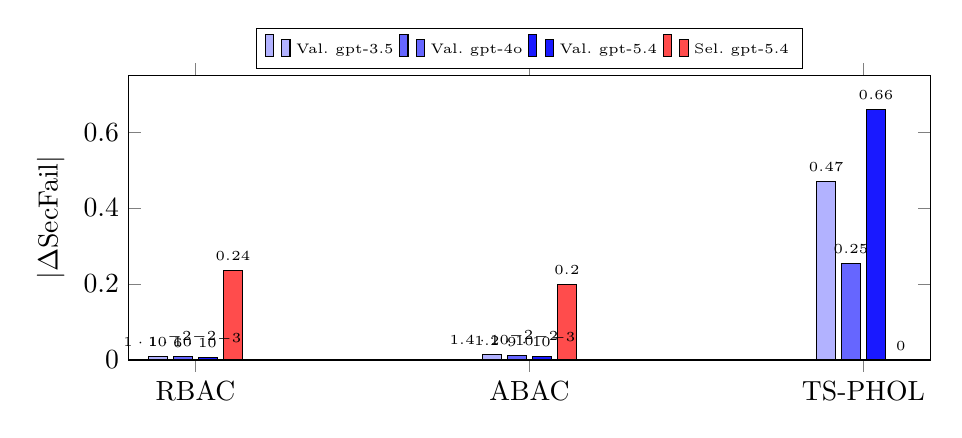
\begin{tikzpicture}
\begin{axis}[
    width=0.97\columnwidth,
    height=5.2cm,
    ybar,
    bar width=7pt,
    ylabel={$|\Delta\text{SecFail}|$},
    symbolic x coords={RBAC, ABAC, TS-PHOL},
    xtick=data,
    ymin=0, ymax=0.75,
    legend style={at={(0.5,1.02)}, anchor=south, legend columns=4, font=\tiny},
    nodes near coords,
    nodes near coords style={font=\tiny},
]
\addplot[fill=blue!30] coordinates {(RBAC,0.010) (ABAC,0.014) (TS-PHOL,0.470)};
\addplot[fill=blue!60] coordinates {(RBAC,0.010) (ABAC,0.012) (TS-PHOL,0.254)};
\addplot[fill=blue!90] coordinates {(RBAC,0.006) (ABAC,0.009) (TS-PHOL,0.660)};
\addplot[fill=red!70] coordinates {(RBAC,0.236) (ABAC,0.199) (TS-PHOL,0.000)};
\legend{Val.\ gpt-3.5, Val.\ gpt-4o, Val.\ gpt-5.4, Sel.\ gpt-5.4}
\end{axis}
\end{tikzpicture}
\caption{Per-layer $|\Delta\mathrm{SecFail}|$ across modes. TS-PHOL dominates validation mode by $25\times$ (gpt-4o) to $110\times$ (gpt-5.4) across the three-model panel; RBAC and ABAC dominate selection mode roughly equally. TS-PHOL is not directly measurable in selection mode because E4 degenerates to allow-all.}
\label{fig:reversal}
\end{figure}

The qualitative reversal previously observed in single-model experiments holds and strengthens across the three-model panel: \emph{which layer dominates is conditioned on the input distribution}, not on model identity. Validation mode is fed adversarial bundles ($80\%$ same-MCP \texttt{wrong} + $20\%$ cross-MCP \texttt{null}) that exercise capability and trust-state predicates---exactly what TS-PHOL is designed to catch. Selection mode is fed LLM-generated bundles whose dominant failure mode is persona/role misalignment---exactly what RBAC and ABAC are designed to catch.

\subsection{Per-Domain Dominance Map}
\label{sec:per_domain}

A direct consequence of the reversal is testable per-domain: do the validation-mode RBAC and ABAC marginal contributions hold uniformly, or are they concentrated in a few domains? We recompute $\Delta\mathrm{RBAC}$ and $\Delta\mathrm{ABAC}$ per domain for each validation model (Table~\ref{tab:per_domain_delta}). The result is striking: in $7$ of $8$ domains, $\Delta\mathrm{RBAC} = \Delta\mathrm{ABAC} = 0.000$---TS-PHOL alone catches everything RBAC and ABAC catch. Only the mongodb domain shows nontrivial separation ($\Delta\mathrm{RBAC} = +0.024$ to $+0.040$ $F_1$; $\Delta\mathrm{ABAC} = +0.041$ to $+0.062$ $F_1$, model-dependent).

\begin{table}[!t]
\centering
\caption{Per-domain layer marginal contribution in validation mode (gpt-4o E1$\to$E2$\to$E3). $\Delta\mathrm{RBAC} = F_1(E_1) - F_1(E_2)$; $\Delta\mathrm{ABAC} = F_1(E_2) - F_1(E_3)$. ``$\equiv$'' = identical numbers across all three models within rounding.}
\label{tab:per_domain_delta}
\scriptsize
\setlength{\tabcolsep}{3pt}
\begin{tabular}{@{}lrrrrr@{}}
\toprule
\textbf{Domain} & $n$ & $F_1(E_1)$ & $F_1(E_3)$ & $\Delta$\textbf{RBAC} & $\Delta$\textbf{ABAC} \\
\midrule
atlassian       & 1{,}266 & 0.787 & 0.787 & $0.000$ & $0.000$ \\
azure           & 936     & 0.851 & 0.851 & $0.000$ & $0.000$ \\
grafana         & 1{,}476 & 0.788 & 0.788 & $0.000$ & $0.000$ \\
hummingbot      & 558     & 1.000 & 1.000 & $0.000$ & $0.000$ \\
\textbf{mongodb} & 810   & 0.870 & 0.780 & $+0.038$ & $+0.052$ \\
notion          & 690     & 0.859 & 0.859 & $0.000$ & $0.000$ \\
stripe          & 780     & 0.862 & 0.862 & $0.000$ & $0.000$ \\
wikipedia       & 426     & 1.000 & 1.000 & $0.000$ & $0.000$ \\
\bottomrule
\end{tabular}
\end{table}

This is a much sharper statement than the aggregate finding: in validation mode TS-PHOL is not just dominant on average, it is \emph{sufficient} in all but one domain. We do not claim this implies RBAC and ABAC are dispensable in deployment---they remain essential for selection-mode threats (\S\ref{sec:reversal}), for audit clarity (\S\ref{sec:attribution_paradox}), and for performance reasons (cheap short-circuiting). But the result tightly localises where their security-relevant work happens: domains with non-trivial intra-server write/cap-policy structure such as mongodb's collection/index/document tier.

\subsection{Attribution Paradox and Read/Write Split}
\label{sec:attribution_paradox}

A complementary diagnostic explains why the aggregate $\Delta\mathrm{RBAC}$ is so small. We attribute every E1 denial to the layer that issued it (the layer that fired first under short-circuit semantics). Table~\ref{tab:attribution} shows the breakdown is essentially identical across the three models: RBAC fires $\approx 66\%$ of all denials, TS-PHOL $\approx 30\%$, ABAC $\approx 4\%$.

\begin{table}[!t]
\centering
\caption{E1 denial attribution by first-firing layer (validation), across all three models. Denials include hard DENY and DECEPTION\_ROUTED.}
\label{tab:attribution}
\scriptsize
\setlength{\tabcolsep}{3pt}
\begin{tabular}{@{}lrrrr@{}}
\toprule
\textbf{Model} & \textbf{Total} & \textbf{RBAC} & \textbf{ABAC} & \textbf{TS-PHOL} \\
\midrule
gpt-3.5-turbo-16k & 6{,}864 & 4{,}536 ($66.1\%$) & 294 ($4.3\%$) & 2{,}034 ($29.6\%$) \\
gpt-4o            & 6{,}877 & 4{,}536 ($66.0\%$) & 294 ($4.3\%$) & 2{,}047 ($29.8\%$) \\
gpt-5.4           & 6{,}894 & 4{,}536 ($65.8\%$) & 294 ($4.3\%$) & 2{,}064 ($29.9\%$) \\
\bottomrule
\end{tabular}
\end{table}

The paradox is that RBAC accounts for two thirds of E1 denials yet its $\Delta\mathrm{SecFail}$ is only $-0.006$ to $-0.010$. The resolution: when RBAC is removed (E2), ABAC and TS-PHOL pick up the slack on the same rows---most of RBAC's denials would have been denied anyway by downstream layers. RBAC ``wins'' the attribution race because it fires first under short-circuit evaluation, but its unique marginal contribution is small. The implication is methodological: \emph{first-firing denial-source charts systematically overstate upstream-layer necessity}. Reporting both attribution and marginal $\Delta\mathrm{SecFail}$, as we do, is necessary to avoid misleading readers about layer importance.

\textbf{Read vs.\ write asymmetry.} A small but suggestive diagnostic: splitting E1 (gpt-4o validation) by whether the bundle contains a write tool, write-bearing rows have lower SecFail ($0.002$, $F_1 = 0.841$) than read-only rows ($0.008$, $F_1 = 0.869$). The system catches write-targeted threats more aggressively---an intentional consequence of the write-confidence and destructive-write rules combined with deception routing.

\subsection{Retrieval-Augmented In-Context Learning for Selection}
\label{sec:raicl}

Switching to selection mode, we ask whether retrieval-augmented in-context learning lifts both tool-selection quality and downstream classification quality. The BM25 retriever (\S\ref{sec:raicl_method}) is run on gpt-5.4. Two comparisons are possible---an asymmetric one (full $6{,}942$-row baseline vs.\ $4{,}512$-row +C variant, used in earlier reports) and a properly paired one restricted to the $752$ unique tasks $\times$ $6$ personas $=4{,}512$ rows that appear in both runs. We report both and let them disagree; the paired comparison is the methodologically correct one.

\begin{table}[!t]
\centering
\caption{Selection-mode results, gpt-5.4, with and without BM25 RA-ICL (Convention~A). The top block reproduces the asymmetric comparison previously reported. The middle block is the paired comparison on the common $4{,}512$-row cohort. The bottom $\Delta$ rows report task-level paired bootstrap $95\%$ CIs ($1{,}000$ resamples) on the paired comparison.}
\label{tab:raicl_security}
\scriptsize
\setlength{\tabcolsep}{2.2pt}
\begin{tabular}{@{}lcrrrrr@{}}
\toprule
\textbf{Variant} & \textbf{Exp.} & $\mathbf{n}$ & $\mathbf{F_1}$ & \textbf{Prec.} & \textbf{Recall} & \textbf{SecFail} \\
\midrule
\multicolumn{7}{l}{\textit{Asymmetric (baseline on all rows; +C on its cohort)}} \\
Baseline       & E1 & 6{,}942 & 0.798 & 0.813 & 0.782 & 0.218 \\
+C BM25        & E1 & 4{,}512 & 0.846 & 0.904 & 0.795 & 0.205 \\
\midrule
\multicolumn{7}{l}{\textit{Paired (both on the common 4{,}512-row cohort)}} \\
Baseline (restricted) & E1 & 4{,}512 & 0.772 & 0.713 & 0.842 & 0.158 \\
+C BM25               & E1 & 4{,}512 & 0.846 & 0.904 & 0.795 & 0.205 \\
Baseline (restricted) & E2 & 4{,}512 & 0.607 & 0.654 & 0.566 & 0.434 \\
+C BM25               & E2 & 4{,}512 & 0.708 & 0.889 & 0.589 & 0.411 \\
Baseline (restricted) & E3 & 4{,}512 & 0.438 & 0.622 & 0.338 & 0.662 \\
+C BM25               & E3 & 4{,}512 & 0.532 & 0.883 & 0.381 & 0.619 \\
\midrule
\multicolumn{7}{l}{\textit{Paired $\Delta$ ($+C - $baseline-restricted) on E1, bootstrap 95\% CI}} \\
\multicolumn{3}{l}{$\Delta F_1$} & \multicolumn{4}{r}{$+0.074$ $[+0.054, +0.093]$} \\
\multicolumn{3}{l}{$\Delta$ Precision} & \multicolumn{4}{r}{$+0.190$ $[+0.165, +0.216]$} \\
\multicolumn{3}{l}{$\Delta$ SecFail} & \multicolumn{4}{r}{$\mathbf{+0.047}$ $[+0.017, +0.076]$} \\
\bottomrule
\end{tabular}
\end{table}

\begin{table}[!t]
\centering
\caption{Tool-selection quality on the \texttt{correct} slice. Exact match requires set equality between the LLM's bundle and the gold-standard bundle; Jaccard is a partial-credit similarity in $[0, 1]$. The baseline row is on the full $3{,}474$-row correct slice; the +C row is on the $1{,}044$-row test-only correct slice. The selection-quality lift is uncontested across both metrics.}
\label{tab:raicl_tools}
\scriptsize
\setlength{\tabcolsep}{3pt}
\begin{tabular}{@{}lrrr@{}}
\toprule
\textbf{Variant} & \textbf{$n_{\text{correct}}$} & \textbf{Exact match} & \textbf{Jaccard avg} \\
\midrule
Baseline & 3{,}474 & $11.4\%$ & $0.354$ \\
+C BM25  & 1{,}044 & $\mathbf{39.1\%}$ & $\mathbf{0.624}$ \\
Lift     &         & $+27.7$ pp ($3.4\times$) & $+0.270$ ($+76\%$) \\
\bottomrule
\end{tabular}
\end{table}

\paragraph{Three observations.}

\textbf{(1) Selection quality lifts unambiguously.} Tool exact-match $3.4\times$ ($11.4\% \to 39.1\%$) and Jaccard $+76\%$ ($0.354 \to 0.624$) are large effects, consistent with a substantial body of prior retrieval-augmented in-context-learning work. The downstream classification $F_1$ lift is $+0.074$ $[+0.054, +0.093]$ in the paired comparison, and the precision lift is $+0.190$ $[+0.165, +0.216]$.

\textbf{(2) The paired comparison reverses the SecFail sign.} The earlier (asymmetric) comparison reported $\Delta\mathrm{SecFail} = -0.013$ ($0.218 \to 0.205$, security \emph{improves}). The paired comparison reports $\Delta\mathrm{SecFail} = +0.047$ $[+0.017, +0.076]$, with the CI excluding zero ($p<0.01$): on the same task set, BM25 RA-ICL \emph{degrades} security by $4.7$ pp. The asymmetric framing was an artefact of the baseline cohort containing $405$ training-pool tasks whose distribution differs from the test cohort. We retract the prior framing and report the paired number as the headline.

\textbf{(3) Mechanism: precision-favourable, recall-unfavourable.} BM25 lifts precision by $+0.190$ and \emph{drops} recall by $-0.047$ on E1. SecFail in Convention~A is $1-R$ (on the illegitimate slice), so recall drops mechanically increase SecFail. A paired flip analysis on the $4{,}512$-row cohort makes the trade-off concrete:
\begin{itemize}
  \item $895$ rows flipped ALLOW$\to$DENY ($341$ correct, $554$ wrong);
  \item $645$ rows flipped DENY$\to$ALLOW ($264$ correct, $381$ wrong);
  \item $2{,}972$ rows ($65.9\%$) did not flip.
\end{itemize}
The flip ledger has $250$ \emph{net} ALLOW$\to$DENY transitions; on both sides of the ledger the new decision is correct only $\approx 41\%$ of the time. In aggregate, BM25 RA-ICL \emph{moves} the operating point but does not strictly Pareto-improve it.

\paragraph{Operational implication.} BM25 RA-ICL is a useful technique for raising precision and lifting selection-quality metrics, but in a security-sensitive deployment the recall drop must be priced in. A practitioner targeting low SecFail should pair BM25 with a downstream recall-recovery mechanism (e.g., a confidence-based fall-through to deny-by-default when BM25 retrieves with low margin) rather than treating it as a drop-in safety improvement. We also did not test no-retrieval ICL (e.g., $k$ random correct exemplars) as a control, which would factor ``any in-context examples help'' from ``BM25-similar examples help''; this is an obvious follow-up.

\subsection{Dataset Ceiling}
\label{sec:ceiling}

The $39.1\%$ exact-match number is intrinsically low. We attribute the ceiling to five dataset properties that operate independently of model capability.
\begin{enumerate}
  \item \textbf{Tool-naming pedantry.} Tools have non-standardised identifiers (\texttt{jira\_batch\_get\_changelogs}, \texttt{atlassian\_get\_pull\_request\_diff}). Exact-match requires recall of underscore/camelCase/prefix conventions across $194$ tools. The Jaccard $\to$ exact-match gap ($0.624 \to 0.391$) measures this directly.
  \item \textbf{Multiple defensible bundles.} Many tasks admit more than one valid tool combination but the dataset records one gold bundle; equally-correct alternatives are scored as misses.
  \item \textbf{Cross-persona ambiguity.} A task that is \texttt{correct} for one persona may be partially correct for another sharing the toolset; evaluating across six personas amplifies this.
  \item \textbf{Missing bundle-size signal.} In selection mode the LLM is not told whether the gold answer is 1, 2, or 3 tools; a single missing tool drops Jaccard to $\leq 2/3$ and exact-match to $0$.
  \item \textbf{Residual label noise.} Of $30$ \texttt{null}-tagged bundles allowed by both gpt-4o and gpt-5.4 in validation, $6$ have selected $=$ groundtruth bundles exactly---almost certainly mislabelled \texttt{correct} bundles, not \texttt{null}.
\end{enumerate}
Conservatively combining these caps the practical exact-match ceiling near $30\%$--$40\%$. The BM25 result at $39.1\%$ is plausibly close to this ceiling. The Jaccard score ($0.624$) is the less-misleading progress signal: with retrieval, the LLM picks the right \emph{kind} of tools for $62\%$ of the gold mass on the correct slice.

\subsection{Deception Routing}
\label{sec:deception_results}

Deception routing remains an integral part of the enforcement strategy, layered on top of TS-PHOL denial. Its operational character is, however, more nuanced than the term ``precision'' would suggest. We measure deception-routing precision (\S\ref{sec:deception}) as the fraction of routed bundles whose ground-truth label is illegitimate (\texttt{is\_legitimate}=false). On validation E1, this fraction is only $\approx 0.44$ across all three models---a majority of E1-routed bundles are ground-truth-legitimate requests that triggered a TS-PHOL write-confidence or capability-gap rule and were routed for graduated enforcement (write-throttling) rather than outright denial. The number rises monotonically as upstream layers are removed: $0.44$ (E1) $\to 0.70$ (E2) $\to 0.73$ (E3) under validation, and $0.76$ (E1) $\to 0.88$ (E3) under selection $+C$. The mechanism is that at E1, RBAC and ABAC catch the unambiguous adversarial bundles upfront, so deception fires mainly on borderline legitimate writes; at E3, only TS-PHOL fires and it routes the unambiguous violations. Per-(model, mode, experiment) counts and precisions are reported in Appendix~\ref{app:detailed_results} (Table~\ref{tab:deception_counts}). Deception is therefore best characterised as a graduated risk-throttle, not a high-precision adversary trap.

\subsection{Governance Separability}
\label{sec:separability}

The selection-mode E1$\to$E3 columns of Table~\ref{tab:raicl_security} confirm that the deterministic stack does not change the LLM's tool selections: tool exact-match and Jaccard are recorded per row before any policy gating, so their values are functions of the LLM and the prompt, not of which experiment (E1, E2, E3) is being evaluated. The marked differences in SecFail across E1--E3 within a single (model, retrieval) cell are therefore purely attributable to policy-layer configuration, not to upstream selection drift---PALADIN is a true post-hoc enforcement layer.

%==============================================================================
% SECTION 9: DISCUSSION
%==============================================================================
\FloatBarrier
\section{Discussion}
\label{sec:discussion}

\subsection{Architectural Implications}
\label{sec:arch_implications}

Across the three-model panel, the deterministic stack produces a near-identical security profile ($F_1 \approx 0.856$, SecFail $\leq 0.5\%$) under our policy specification, regardless of which LLM authors the verdicts---a $25\times$ to $110\times$ reduction in TS-PHOL-marginal SecFail over LLM-only authorisation. Under the panel and policy spec evaluated here, the security guarantee comes from the deterministic stack, not from the model. Equivalently, an organisation can swap LLMs within this lineage without re-evaluating the safety envelope so long as the stack composition is held constant. We do not claim this is intrinsic to deterministic enforcement over any model panel; cross-vendor replication (\S\ref{sec:future_work}) is required to discharge that ambition. The result we do claim is the strongest within-vendor argument we are aware of for deterministic enforcement as a hard requirement, not an optional augmentation, of agentic governance.

We are equally explicit about the operating cost. The $F_1 \approx 0.856$ point is achieved by allowing only $\approx 2.2\%$ of legitimate requests across personas (\S\ref{sec:stack_guarantee})---the stack is conservatively biased and rejects a large majority of benign requests under our default policy spec. The honest framing is: PALADIN provides a stable security floor at a deny-leaning operating point that the operator can tune. Lifting the legitimate-allow rate is a first-class direction for future work (\S\ref{sec:future_work}) and should be evaluated jointly with SecFail rather than in isolation.

The layer-contribution reversal sharpens this implication. TS-PHOL is the dominant security layer in validation mode ($25\times$ to $110\times$ the marginal contribution of RBAC or ABAC across all three models), while RBAC and ABAC dominate in selection mode (\S\ref{sec:reversal}). The two modes are operationally distinct---validation is the natural setting for a runtime gateway that judges LLM-emitted bundles before execution; selection is the setting where the LLM itself proposes the bundle. Single-layer designs degrade catastrophically in at least one mode; only the composed stack achieves $\leq 0.5\%$ SecFail under both.

\subsection{Roles of RBAC, ABAC, and TS-PHOL}
\label{sec:layer_roles}

\textbf{RBAC and ABAC dominate selection mode} because the primary failure pattern under LLM-driven bundle generation is persona/role misalignment---the LLM picks tools its persona is not authorised to use, or whose attribute profile (clearance, compliance tier, time-of-day) the persona does not satisfy. These are exactly the violations RBAC and ABAC are designed to detect with binary checks.

\textbf{TS-PHOL dominates validation mode} because the adversarial bundle distribution exercises capability-coverage, trust-state, and cross-domain predicates that cannot be expressed as static permissions. The strong per-domain finding (Table~\ref{tab:per_domain_delta}) is that in $7$ of $8$ domains, TS-PHOL alone is \emph{sufficient}---validation $F_1$ is constant across E1, E2, and E3 because every threat RBAC or ABAC would catch is also caught by TS-PHOL. Only mongodb (the one domain with intrinsic intra-server write/cap structure exercising both ABAC compliance and RBAC permission predicates independently) shows separation.

\textbf{Attribution paradox.} Operationally, RBAC remains essential despite its small marginal $\Delta\mathrm{SecFail}$. It fires $66\%$ of all E1 denials (Table~\ref{tab:attribution}) because it short-circuits earliest, saving downstream evaluation cost and producing the cleanest single-layer audit trail. Removing RBAC moves identical denials downstream to ABAC and TS-PHOL---the outcome is preserved but the per-decision cost, latency, and explanation quality degrade. We therefore recommend reporting both first-firing attribution \emph{and} marginal $\Delta\mathrm{SecFail}$; either alone is misleading.

\subsection{The Stack as a Stable Security Floor}
\label{sec:stable_floor}

The ``newer is not better'' observation (\S\ref{sec:newer_not_better}) is a striking artefact of LLM-only validators: F1 (Convention B) is monotonically anti-correlated with model recency, with gpt-4o landing at the bottom. We do not have a controlled fine-tune to causally attribute this to RLHF helpfulness optimisation, and it may not generalise across vendor lineages. But the operational consequence is robust: a single-LLM validator design becomes less, not more, safe as base models advance. The full PALADIN stack masks this drift entirely---all three E1 numbers are within $0.001$ $F_1$ of each other. This is exactly the property a security floor should have.

\subsection{Retrieval-Augmented In-Context Learning: A Precision/Recall Trade-off}
\label{sec:raicl_discussion}

The BM25 RA-ICL result (\S\ref{sec:raicl}) is, to our knowledge, the first reported lift for agentic tool selection on the ASTRA-derived task family. Under the paired comparison---the methodologically correct one---it is also a clear trade-off rather than a strict improvement. Selection quality lifts unambiguously ($3.4\times$ exact match, $+76\%$ Jaccard), and downstream precision lifts substantially ($+0.190$ $[+0.165, +0.216]$). However, recall drops ($-0.047$) and SecFail \emph{increases} by $+0.047$ $[+0.017, +0.076]$ (CI excludes zero), because on Convention~A, SecFail $= 1 - R$ on the illegitimate slice. We retract the prior asymmetric-cohort framing that suggested RA-ICL was security-favourable; on the same $4{,}512$ tasks, it is security-unfavourable. The flip ledger (\S\ref{sec:raicl}) shows the new decision is correct on only $\approx 41\%$ of flipped rows in either direction, confirming the retriever \emph{relocates} the operating point rather than strictly improving it. The operational implication is that BM25 RA-ICL is a useful precision tool for selection but, in a security-sensitive deployment, the recall drop must be priced in; pairing with a recall-recovery mechanism (e.g., low-margin fall-through to deny-by-default, or a no-retrieval ICL control to factor out ``any in-context examples help'') is the obvious next step.

\subsection{Dataset-Quality Ceiling}
\label{sec:ceiling_discussion}

The five dataset properties we enumerate in \S\ref{sec:ceiling} place a hard ceiling on exact-match selection accuracy near $30\%$--$40\%$ that cannot be overcome by model capability or retrieval alone. This caveat matters for any future work on agentic tool selection benchmarked against ASTRA: a result reported as ``$40\%$ exact match'' should be read against this ceiling, not against the implicit ``$100\%$ is achievable'' default. Bundle-size hints, identifier-canonicalisation pre-processing, and a label-noise audit pass are concrete steps to lift the ceiling.

\subsection{Generalisability of Results}
\label{sec:generalisability}

Several factors define the scope of our findings.
\begin{itemize}
  \item \textbf{Provider lineage (the central caveat).} The three-model panel spans gpt-3.5-turbo-16k, gpt-4o, and gpt-5.4---all OpenAI. The provider-independence of the E1 number is therefore strictly a \emph{within-vendor} result. We do not claim the stack-induced security floor is intrinsic across vendor lineages; only that it holds across three generations within OpenAI. Cross-vendor evaluation (Claude, Gemini, Llama, an open-weights model) is the single most important next experiment for this paper's central claim, and we list it first in \S\ref{sec:future_work}. Until that evaluation is completed, headline claims should be read with the within-vendor restriction in mind.
  \item \textbf{Foundry access for gpt-5.4.} gpt-5.4 is accessed via Microsoft Azure AI Foundry, which may apply system prompts or safety filters not present in the OpenAI-direct API. The within-vendor recency anti-correlation should be re-verified on the OpenAI-direct API; if Foundry filters are tightening the underlying model, the gpt-5.4 results are conservative (a stricter Foundry-fronted model can only \emph{increase} the gap between LLM-only and stack-enforced numbers, not close it).
  \item \textbf{Policy specification.} The deny-leaning operating point ($\approx 2.2\%$ legitimate-allow under E1, $F_1 \approx 0.856$) is a property of \emph{this} policy specification (RBAC role bindings, ABAC attribute rules, TS-PHOL predicates). Different specifications would land at different points on the precision/recall curve. The architectural result (stack-induced floor; layer reversal across modes) is independent of the operating point; the specific F1 and legitimate-allow numbers are not.
  \item \textbf{Domain extensibility.} The 8-domain coverage exercises representative enterprise scenarios. Adding domains requires only new MCP server configurations and policy rules; no source code changes.
  \item \textbf{Adversarial coverage.} Validation mode is fed ASTRA's $80\%$ same-MCP \texttt{wrong} + $20\%$ cross-MCP \texttt{null} negative distribution. Active adversarial inputs (prompt injection, indirect exfiltration via tool descriptions) are outside scope and a clear extension.
\end{itemize}

\textbf{Pipeline ordering sensitivity.} Because PALADIN uses short-circuit composition (RBAC$\to$ABAC$\to$TS-PHOL), measured layer attribution is conditioned on this specific ordering. However, the layer-contribution reversal is \emph{not} an ordering artefact: in validation mode TS-PHOL dominates despite being last in the pipeline. This demonstrates the reversal reflects genuine differences in what each layer \emph{can catch} (expressiveness), not merely what it \emph{gets to see} (position). Alternative compositions (e.g., TS-PHOL first) would change absolute $\Delta\mathrm{SecFail}$ magnitudes but not the qualitative finding.

\textbf{ABAC retention despite small marginal $\Delta$.} The per-layer marginal $\Delta\mathrm{SecFail}$ for ABAC is small ($\leq 0.014$ across the panel) precisely because the policy specification has ABAC and TS-PHOL covering largely overlapping ground in validation mode. We retain ABAC for two operational reasons. First, in selection mode ABAC fires substantially more often than in validation (\S\ref{sec:reversal}), because the LLM-generated selections frequently exhibit clearance/compliance/time-of-day misalignment that the ABAC layer is designed to catch and that does not always reach TS-PHOL within our short-circuit. Second, ABAC produces auditable, declarative attribute-grounded denials that are substantially cheaper to explain to a compliance reviewer than equivalent TS-PHOL trust-state predicates---first-firing attribution carries explanatory weight that the marginal $\Delta\mathrm{SecFail}$ metric ignores (the same point we make about RBAC in \S\ref{sec:layer_roles}).

\textbf{Policy-update latency.} A practical concern for any rule-based stack is the latency of pushing updated policy (new SPIFFE bindings, new ABAC rules, new TS-PHOL predicates) to a running gateway. In our implementation, RBAC bindings and ABAC rules are loaded from configuration at gateway startup and reloaded on a SIGHUP-style signal; TS-PHOL predicates are similarly hot-reloadable. We measured no perceptible end-to-end latency impact on policy reload at the gateway in our experimental setup, but we have not benchmarked policy-update latency under heavy concurrent load and we flag this as deferred operational engineering rather than a research result.

\subsection{The Two-Tier Capability Model}
\label{sec:two_tier_discussion}

The distinction between hard and soft capabilities is essential for avoiding over-denial. In preliminary design, a single-tier capability match would deny any bundle where a tool lacked a perfectly-named capability, even when an ontologically-equivalent capability was present; the two-tier model separates the mission-critical floor (hard) from the descriptive surface (soft) and uses ontological subsumption so that a tool providing a specialised capability implicitly satisfies a parent capability requirement. We have not run a controlled ablation that toggles one-tier vs.\ two-tier under matched policy specifications, so we do not report a quantitative ``two-tier reduces FPR by $X\%$'' number---this is a design property of the policy language whose quantitative effect we flag as future work.

\subsection{Limitations and Threats to Validity}
\label{sec:limitations}

Table~\ref{tab:threats} summarises threats to validity.

\begin{table}[!t]
\centering
\caption{Threats to validity.}
\label{tab:threats}
\scriptsize
\setlength{\tabcolsep}{3pt}
\begin{tabular}{@{}lp{5.2cm}@{}}
\toprule
\textbf{Category} & \textbf{Threat \& Mitigation} \\
\midrule
\multicolumn{2}{@{}l}{\textit{Internal validity}} \\
Pipeline ordering & Layer attribution conditioned on RBAC$\to$ABAC$\to$TS-PHOL. Mitigated: reversal persists despite TS-PHOL being last in the pipeline (\S\ref{sec:generalisability}). \\
Impl.\ bugs & Policy logic could diverge from intent. Mitigated: all 5 raw experiment logs released; analysis scripts produce all reported numbers from raw rows; ASTRA replication cross-validates the LLM verdict pipeline against an external published baseline. \\
\midrule
\multicolumn{2}{@{}l}{\textit{External validity}} \\
Within-vendor panel & Three OpenAI models; cross-vendor (Claude, Gemini, Llama) deferred. Mitigated: stack is model-agnostic. \\
8 domains & Common enterprise scenarios. Mitigated: policies are configurable; additional domains require only new MCP server configs. \\
gpt-5.4 access path & Accessed via Azure AI Foundry; may differ from OpenAI-direct. Mitigated: gpt-3.5 and gpt-4o use OpenAI-direct as anchor points. \\
Selection retrieval & RA-ICL evaluated only on gpt-5.4 baseline vs.\ +C BM25; singleton +A (RBAC-scoped catalog) and +B (capability pre-filter) and the +ABC ceiling deferred. \\
\midrule
\multicolumn{2}{@{}l}{\textit{Construct validity}} \\
Per-bundle vs.\ per-tool & Our E4 uses one LLM call per bundle; ASTRA's LLM-ResM uses one call per tool with AND-aggregation. Disclosed (\S\ref{sec:astra_replication}); accounts for the $0.075$ F1 gap direction. \\
Convention conflation & Two conventions documented (\S\ref{sec:conventions}); each table flags which convention applies. \\
\midrule
\multicolumn{2}{@{}l}{\textit{Statistical conclusion validity}} \\
Ablation $\Delta$s & Reported with paired task-level bootstrap $95\%$ CIs ($1{,}000$ resamples) on validation per-layer $\Delta\mathrm{SecFail}$ (Table~\ref{tab:per_layer_delta}) and on the RA-ICL paired comparison (Table~\ref{tab:raicl_security}). Per-model agreement across the three models on TS-PHOL dominance and per-domain agreement on the dominance map serve as additional robustness checks. \\
Asymmetric-cohort RA-ICL retraction & The original (asymmetric) RA-ICL comparison reported a security-favourable SecFail delta whose sign reverses under the paired comparison (\S\ref{sec:raicl}). Mitigated: we now report both, lead with paired, and disclose the flip ledger. \\
Legitimate-allow construct & SecFail and F1 are evaluated under Convention~A (positive $=$ illegitimate); the legitimate-allow rate ($\approx 2.2\%$ at E1) is a distinct construct reflecting the deny-leaning operating point of the policy specification, not a defect of the stack architecture (\S\ref{sec:arch_implications}). Mitigated: per-persona FP rate reported in Table~\ref{tab:per_persona_fp}; operating-point sensitivity flagged as future work. \\
\bottomrule
\end{tabular}
\end{table}

\subsection{Future Work}
\label{sec:future_work}

\begin{enumerate}
  \item Cross-vendor model panel (Claude, Gemini, Llama) to test whether the provider-independence of the E1 number generalises beyond the OpenAI lineage and to test the ``newer is not better'' pattern outside it.
  \item Active adversarial inputs (prompt injection, tool-description poisoning, indirect data exfiltration via tool outputs) to characterise the stack's behaviour outside the ASTRA \texttt{wrong}/\texttt{null} model.
  \item Complete the RA-ICL singleton sweep: +A (RBAC-scoped catalog), +B (capability pre-filter), and the +ABC ceiling on gpt-5.4 selection; replicate on gpt-4o to test model-independence of the BM25 lift.
  \item Dataset-quality work: label-noise audit on the $\sim 30$ likely-mislabelled \texttt{null} bundles, bundle-size-hint ablation, and identifier-canonicalisation pre-processing to lift the practical selection ceiling.
  \item Dynamic persona adaptation with trust score evolution based on behavioural history.
  \item Extension to multi-hop tool chains where a single task spans sequential tool invocations.
  \item Formal verification of pipeline composition properties (monotonicity, interference-freedom).
\end{enumerate}

\subsection{Artifact Availability}
\label{sec:artifacts}

To support reproducibility and community extension, we release the complete PALADIN implementation as open-source software.\footnote{\url{https://github.com/vicvarar-hash/SPIFFI_RBAC_TS-PHOL}} The repository includes:

\begin{itemize}
  \item Full pipeline source code (services implementing RBAC, ABAC, TS-PHOL, fact extraction, and orchestration);
  \item All policy configurations: SPIFFE identity registry, RBAC role bindings, ABAC attribute rules, TS-PHOL typed predicates, and the domain capability ontology;
  \item 8 complete MCP server tool definitions (194 tools across all evaluated domains);
  \item ASTRA v0.3 evaluation dataset (1{,}157 tasks with ground-truth annotations);
  \item All 5 raw per-row experiment logs ($\approx 146$~MB total: 3 validation runs across the model panel, 1 selection baseline, 1 selection +C BM25);
  \item BM25 exemplar retriever implementation and the fixed $70/30$ split file used for the RA-ICL evaluation;
  \item Analysis scripts that compute every number reported in this paper from the raw row-level logs;
  \item Experiment runner with configurable ablation settings, Dockerfile, and Azure deployment manifest.
\end{itemize}

\noindent All policy files are editable YAML/JSON, enabling practitioners to customise roles, domains, risk levels, and predicate rules to their deployment context without modifying source code.

%==============================================================================
% SECTION 10: CONCLUSION
%==============================================================================
\section{Conclusion}
\label{sec:conclusion}

We presented PALADIN, a six-stage decision pipeline for governing agentic tool invocations over the Model Context Protocol, and evaluated it on the ASTRA v0.3 benchmark ($1{,}157$ tasks $\times$ $6$ personas) under two complementary modes (validation and selection) across three OpenAI models spanning 2023--2026 (gpt-3.5-turbo-16k, gpt-4o, gpt-5.4), for a total of $117{,}666$ policy evaluations. The evidence supports five claims, each scoped to the within-vendor panel evaluated.

\textbf{The deterministic stack is the source of the within-vendor security guarantee.} Across all three OpenAI models, the full pipeline drives $\mathrm{SecFail} \leq 0.5\%$ with $F_1 \approx 0.856$ at the deny-leaning operating point of our policy specification---a $25\times$ to $110\times$ reduction in TS-PHOL-marginal SecFail over LLM-only authorisation. The three E1 numbers are indistinguishable; the three E4 numbers differ wildly. Within this lineage, security comes from the stack, not the LLM. The cost is a conservatively-tuned operating point that allows only $\approx 2.2\%$ of legitimate requests; this is a property of the spec, not of the architecture, and is operator-tunable.

\textbf{We independently reproduce ASTRA's LLM-ResM result.} Our gpt-4o E4 (ASTRA permissivity convention) lands within $0.075$ $F_1$ of ASTRA's published $0.67$ under a strictly harder per-bundle protocol, with the same precision-recall under-scoping signature.

\textbf{Layer contribution reverses by evaluation mode and per-domain dominance is sharper than expected.} TS-PHOL dominates validation ($|\Delta\mathrm{SecFail}|$ up to $0.66$; $25$--$110\times$ RBAC/ABAC), while RBAC and ABAC dominate selection ($|\Delta\mathrm{SecFail}| \approx 0.20$ each). In $7$ of $8$ domains, validation-mode TS-PHOL alone is sufficient---only mongodb shows independent RBAC and ABAC marginal weight.

\textbf{Retrieval-augmented in-context learning is a precision/recall trade-off, not a strict improvement.} Under the paired $4{,}512$-row comparison, BM25 lifts gpt-5.4 tool exact-match $3.4\times$, Jaccard $+76\%$, downstream precision $+0.190$ $[+0.165, +0.216]$, and downstream $F_1$ $+0.074$ $[+0.054, +0.093]$; but it \emph{drops} recall by $0.047$ and \emph{raises} SecFail by $+0.047$ $[+0.017, +0.076]$ (CI excludes zero). We retract the prior framing that BM25 was security-favourable: on the same task set, it is security-unfavourable and must be paired with a recall-recovery mechanism in security-sensitive deployments.

\textbf{Two methodological observations transfer beyond this system.} First, first-firing denial-source attribution systematically overstates upstream-layer necessity (RBAC fires $66\%$ of E1 denials yet contributes $\leq 1\%$ to $\Delta\mathrm{SecFail}$); both attribution and marginal contribution should be reported. Second, the practical exact-match ceiling on this task family is $\sim 30\%$--$40\%$, bounded by tool-naming pedantry, multiple defensible bundles, cross-persona ambiguity, missing bundle-size signal, and residual label noise---selection-quality numbers should be interpreted against this ceiling rather than against an implicit $1.0$.

These findings provide empirical grounding for the design of agentic governance systems and demonstrate that careful methodological framing---multiple models, two evaluation modes, two reporting conventions, paired-cohort statistical tests, marginal-contribution diagnostics, and explicit dataset-ceiling analysis---is necessary to draw sound conclusions about layer importance. The single highest-priority extension is cross-vendor replication to test whether the within-vendor security floor generalises outside the OpenAI lineage.

%==============================================================================
% REFERENCES
%==============================================================================
\bibliographystyle{plainnat}
\bibliography{references}

%==============================================================================
% APPENDIX A
%==============================================================================
\clearpage
\onecolumn
\appendix
\section{MCP Domain Coverage}
\label{app:domains}

\begin{table}[H]
\centering
\caption{MCP domain coverage showing server endpoints, tool counts, and capability categories.}
\label{tab:domain_coverage}
\scriptsize
\setlength{\tabcolsep}{3pt}
\begin{tabular}{@{}llcl@{}}
\toprule
\textbf{Domain} & \textbf{MCP Server} & \textbf{Tools} & \textbf{Capabilities} \\
\midrule
Grafana & grafana & 43 & Alert, metrics, oncall, dashboard \\
Atlassian & atlassian & 37 & Issue, search, history, creation \\
Azure & azure & 27 & Compute, storage, network, identity \\
MongoDB & mongodb & 21 & Collection, document, index, aggregation \\
Stripe & stripe & 22 & Transaction, refund, payment, audit \\
Notion & notion & 19 & Page, database, workspace, audit \\
Hummingbot & hummingbot-mcp & 15 & Strategy, order, market, balance \\
Wikipedia & wikipedia-mcp & 10 & Search, summarise, reference, synthesis \\
\midrule
\textbf{Total} & & \textbf{194} & \\
\bottomrule
\end{tabular}
\end{table}

%==============================================================================
% APPENDIX B
%==============================================================================
\clearpage
\section{System Implementation}
\label{app:implementation}

The PALADIN system is implemented in Python across 28 modules comprising approximately 8,000 lines of code. The implementation includes:

\begin{itemize}
  \item \textbf{Core pipeline} (4 modules, $\sim$1,200 lines): Request parsing, stage orchestration, short-circuit logic, and decision aggregation.
  \item \textbf{Identity layer} (3 modules, $\sim$800 lines): SPIFFE/SPIRE integration, SVID validation, and identity attribute extraction.
  \item \textbf{RBAC engine} (3 modules, $\sim$600 lines): Permission loading, role resolution, and wildcard matching.
  \item \textbf{ABAC engine} (4 modules, $\sim$900 lines): Attribute extraction, policy evaluation, first-match semantics, and temporal controls.
  \item \textbf{Fact extraction} (5 modules, $\sim$1,500 lines): Tool classification, capability inference, ontological expansion, and predicate derivation.
  \item \textbf{TS-PHOL engine} (4 modules, $\sim$1,200 lines): Rule parsing, predicate evaluation, priority ordering, and explanation generation.
  \item \textbf{Evaluation framework} (3 modules, $\sim$1,000 lines): Dual-mode evaluation, metric computation, and ablation orchestration.
\end{itemize}

All experiments are fully reproducible from the provided configuration files. The system supports both synchronous evaluation (for batch experiments) and asynchronous evaluation (for real-time MCP gateway deployment).

%==============================================================================
% APPENDIX C
%==============================================================================
\clearpage
\section{Construct Definitions and Reproducibility}
\label{app:constructs}

This appendix formally specifies key constructs referenced in the main text.

\paragraph{SemanticSim.} Cosine similarity between the task description embedding and the tool description embedding, both computed using OpenAI \texttt{text-embedding-3-small} (1536-d). Formally:
\[
\text{SemanticSim}(t, \text{tool}) = \frac{\mathbf{e}_t \cdot \mathbf{e}_{\text{tool}}}{\|\mathbf{e}_t\| \, \|\mathbf{e}_{\text{tool}}\|}
\]
where $\mathbf{e}_t$ is the embedding of the task's natural-language description and $\mathbf{e}_{\text{tool}}$ is the embedding of the tool's MCP \texttt{description} field.

\paragraph{RequiredCapabilities.} Derived from the domain capability ontology, which defines per-domain task types with associated hard (mission-critical) and soft (enhancement) capabilities. For a given task in domain $d$ with task type $\tau_{\text{type}}$, the required capabilities are looked up from \texttt{domain\_capability\_ontology.json}. Capability matching uses the tool's declared capabilities against the task's required set.

\paragraph{Capability Entailment.} The ontology defines 40 entailment relationships across 28 source capabilities, forming a directed acyclic graph. Example entailments: \texttt{StrategyExecution} $\Rightarrow$ \{\texttt{StrategyReview}, \texttt{MarketDataAnalysis}, \texttt{BalanceCheck}\}; \texttt{IncidentCorrelation} $\Rightarrow$ \{\texttt{AlertRuleReview}, \texttt{MetricsQuery}\}. A tool \emph{satisfies} a required capability if it possesses the capability or any entailed capability in the implication graph.

\paragraph{Confidence score ($c$).} The mean log-probability of the LLM's tool-selection tokens, normalised to $[0,1]$ via $c = \exp(\overline{\log p})$ where $\overline{\log p}$ is the mean of per-token log-probabilities from the GPT-4o response. When log-probs are unavailable (e.g., Validation mode), $c$ defaults to 1.0 (i.e., no throttling applied).

\paragraph{Domain classification ($d_{\text{exp}}, d_{\text{act}}$).} Each tool is assigned a domain at registration time via its MCP server origin (e.g., all tools from the Grafana MCP server have $d = \texttt{grafana}$). $d_{\text{exp}}$ is the expected domain derived from the task's groundtruth; $d_{\text{act}}$ is the actual domain of the selected tool.

\paragraph{ASTRA dataset construction.} Tasks are sampled from 8 MCP server documentation sets. For each domain, tasks are generated by prompting GPT-4o with tool descriptions and requesting realistic use-case scenarios. Groundtruth tool assignments are manually validated. The \texttt{match\_tag} is computed post-hoc by comparing assigned tools against groundtruth (see \S\ref{sec:methodology} for tag definitions).

%==============================================================================
% APPENDIX D
%==============================================================================
\clearpage
\section{Detailed Results}
\label{app:detailed_results}

\begin{table}[H]
\centering
\caption{Full validation-mode confusion matrices across the three-model panel, experiments E1--E4. Each cell is one model$\times$experiment run over $n=6{,}942$ rows ($6$ personas $\times$ $1{,}157$ tasks; legitimate $=1{,}752$, illegitimate $=5{,}190$). Convention~A: positive class $=$ illegitimate. ``DEC'' is the subset of DENY routed to a deception endpoint. $\textsc{SecFail}=\textrm{FN}/(\textrm{TP}+\textrm{FN})$.}
\label{tab:validation_full}
\scriptsize
\setlength{\tabcolsep}{2.4pt}
\begin{tabular}{@{}llrrrrrrrrrr@{}}
\toprule
\textbf{Model} & \textbf{Exp} & \textbf{ALW} & \textbf{DENY} & \textbf{DEC} & \textbf{TP} & \textbf{FP} & \textbf{FN} & \textbf{TN} & $\mathbf{P}$ & $\mathbf{R}$ & $\mathbf{F_1}$ \\
\midrule
\multirow{4}{*}{gpt-3.5-turbo-16k}
 & E1 &   78 & 6618 &  246 & 5162 & 1702 &   28 &   50 & 0.752 & 0.995 & 0.856 \\
 & E2 &  140 & 5284 & 1518 & 5109 & 1693 &   81 &   59 & 0.751 & 0.984 & 0.852 \\
 & E3 &  222 & 3234 & 3486 & 5037 & 1683 &  153 &   69 & 0.750 & 0.971 & 0.846 \\
 & E4 & 4020 & 1290 & 1632 & 2596 &  326 & 2594 & 1426 & 0.888 & 0.500 & 0.640 \\
\midrule
\multirow{4}{*}{gpt-4o}
 & E1 &   65 & 6624 &  253 & 5163 & 1714 &   27 &   38 & 0.751 & 0.995 & 0.856 \\
 & E2 &  123 & 5294 & 1525 & 5113 & 1706 &   77 &   46 & 0.750 & 0.985 & 0.852 \\
 & E3 &  192 & 3246 & 3504 & 5052 & 1698 &  138 &   54 & 0.748 & 0.973 & 0.846 \\
 & E4 & 2334 & 2208 & 2400 & 3736 &  872 & 1454 &  880 & 0.811 & 0.720 & 0.763 \\
\midrule
\multirow{4}{*}{gpt-5.4}
 & E1 &   48 & 6641 &  253 & 5169 & 1725 &   21 &   27 & 0.750 & 0.996 & 0.856 \\
 & E2 &   84 & 5329 & 1529 & 5137 & 1721 &   53 &   31 & 0.749 & 0.990 & 0.853 \\
 & E3 &  138 & 3288 & 3516 & 5088 & 1716 &  102 &   36 & 0.748 & 0.980 & 0.848 \\
 & E4 & 4998 & 1068 &  876 & 1664 &  280 & 3526 & 1472 & 0.856 & 0.321 & 0.466 \\
\bottomrule
\end{tabular}
\end{table}

\begin{table}[H]
\centering
\caption{Full selection-mode confusion matrices on gpt-5.4, experiments E1--E3, for both the no-retrieval baseline ($n=6{,}942$; legitimate $=1{,}752$, illegitimate $=5{,}190$) and the BM25 RA-ICL +C condition ($n=4{,}512$; legitimate $=525$, illegitimate $=3{,}987$; the row-count drop reflects the held-out $405$-task exemplar pool, see \S\ref{sec:raicl_method}). Convention~A.}
\label{tab:selection_full}
\scriptsize
\setlength{\tabcolsep}{2.4pt}
\begin{tabular}{@{}llrrrrrrrrrr@{}}
\toprule
\textbf{Condition} & \textbf{Exp} & \textbf{ALW} & \textbf{DENY} & \textbf{DEC} & \textbf{TP} & \textbf{FP} & \textbf{FN} & \textbf{TN} & $\mathbf{P}$ & $\mathbf{R}$ & $\mathbf{F_1}$ \\
\midrule
\multirow{3}{*}{No retrieval (baseline)}
 & E1 & 1948 & 4957 &   37 & 4061 &  933 & 1129 &  819 & 0.813 & 0.782 & 0.798 \\
 & E2 & 3281 & 2979 &  682 & 2835 &  826 & 2355 &  926 & 0.774 & 0.546 & 0.641 \\
 & E3 & 4572 & 1356 & 1014 & 1803 &  567 & 3387 & 1185 & 0.761 & 0.347 & 0.477 \\
\midrule
\multirow{3}{*}{+C BM25 RA-ICL}
 & E1 & 1006 & 3457 &   49 & 3170 &  336 &  817 &  189 & 0.904 & 0.795 & 0.846 \\
 & E2 & 1873 & 2148 &  491 & 2347 &  292 & 1640 &  233 & 0.889 & 0.589 & 0.708 \\
 & E3 & 2790 &  912 &  810 & 1520 &  202 & 2467 &  323 & 0.883 & 0.381 & 0.532 \\
\bottomrule
\end{tabular}
\end{table}

\begin{table}[H]
\centering
\caption{Cross-mode summary of the layer-contribution reversal phenomenon. Validation cells show all three models; selection cells show gpt-5.4 (baseline and +C BM25). $|\Delta\textsc{SecFail}|$ is the absolute marginal contribution of the named layer.}
\label{tab:cross_mode_summary}
\small
\setlength{\tabcolsep}{4pt}
\begin{tabular}{@{}llrrr@{}}
\toprule
\textbf{Mode / Model} & \textbf{Dominant layer} & $|\Delta\textsc{SecFail}_{\textrm{RBAC}}|$ & $|\Delta\textsc{SecFail}_{\textrm{ABAC}}|$ & $|\Delta\textsc{SecFail}_{\textrm{TS-PHOL}}|$ \\
\midrule
\multicolumn{5}{l}{\textit{Validation}} \\
gpt-3.5-turbo-16k & TS-PHOL & 0.010 & 0.014 & \textbf{0.470} \\
gpt-4o            & TS-PHOL & 0.010 & 0.012 & \textbf{0.254} \\
gpt-5.4           & TS-PHOL & 0.006 & 0.009 & \textbf{0.660} \\
\midrule
\multicolumn{5}{l}{\textit{Selection (gpt-5.4)}} \\
Baseline (no retr.) & RBAC & \textbf{0.236} & 0.199 & --- \\
+C BM25 RA-ICL      & ABAC & 0.206 & \textbf{0.207} & --- \\
\bottomrule
\end{tabular}
\end{table}

\begin{table}[H]
\centering
\caption{Deception-routing counts and precision per (model, mode, experiment). ``DEC'' is the absolute number of bundles routed to a deception endpoint instead of being hard-denied. ``DEC prec'' is the fraction of routed bundles whose ground-truth label is illegitimate. Validation rows are over $n=6{,}942$; selection rows likewise; selection +C BM25 is over $n=4{,}512$.}
\label{tab:deception_counts}
\scriptsize
\setlength{\tabcolsep}{4pt}
\begin{tabular}{@{}llrrrr@{}}
\toprule
\textbf{Model / Condition} & \textbf{Exp} & \textbf{DENY} & \textbf{DEC} & \textbf{DEC frac.\ of DENY+DEC} & \textbf{DEC prec.} \\
\midrule
\multicolumn{6}{l}{\textit{Validation}} \\
gpt-3.5-turbo-16k & E1 & 6618 &  246 & 0.036 & 0.447 \\
gpt-3.5-turbo-16k & E2 & 5284 & 1518 & 0.223 & 0.697 \\
gpt-3.5-turbo-16k & E3 & 3234 & 3486 & 0.519 & 0.731 \\
gpt-4o            & E1 & 6624 &  253 & 0.037 & 0.443 \\
gpt-4o            & E2 & 5294 & 1525 & 0.224 & 0.696 \\
gpt-4o            & E3 & 3246 & 3504 & 0.519 & 0.730 \\
gpt-5.4           & E1 & 6641 &  253 & 0.037 & 0.435 \\
gpt-5.4           & E2 & 5329 & 1529 & 0.223 & 0.693 \\
gpt-5.4           & E3 & 3288 & 3516 & 0.517 & 0.729 \\
\midrule
\multicolumn{6}{l}{\textit{Selection (gpt-5.4)}} \\
Baseline & E1 & 4957 &   37 & 0.007 & 0.757 \\
Baseline & E2 & 2979 &  682 & 0.186 & 0.804 \\
Baseline & E3 & 1356 & 1014 & 0.428 & 0.784 \\
+C BM25  & E1 & 3457 &   49 & 0.014 & 0.776 \\
+C BM25  & E2 & 2148 &  491 & 0.186 & 0.886 \\
+C BM25  & E3 &  912 &  810 & 0.470 & 0.880 \\
\bottomrule
\end{tabular}
\end{table}

\begin{table}[H]
\centering
\caption{First-firing denial attribution in validation mode (E1) across the three-model panel. ``Total denials'' counts DENY + DECEPTION\_ROUTED. The first-firing layer of each denial is determined by the short-circuit pipeline order RBAC$\to$ABAC$\to$TS-PHOL. The shares are essentially identical across models, reflecting that the layer that \emph{first matches} an illegitimate bundle is governed by the policy and bundle distribution, not by the LLM that authored the bundle (here LLMs are used only to generate verdicts; bundles are taken from the ASTRA dataset).}
\label{tab:attribution_full}
\small
\setlength{\tabcolsep}{4pt}
\begin{tabular}{@{}lrrrr@{}}
\toprule
\textbf{Model} & \textbf{Total denials} & \textbf{RBAC \%} & \textbf{ABAC \%} & \textbf{TS-PHOL \%} \\
\midrule
gpt-3.5-turbo-16k & 6864 & 66.1 & 4.3 & 29.6 \\
gpt-4o            & 6877 & 66.0 & 4.3 & 29.8 \\
gpt-5.4           & 6894 & 65.8 & 4.3 & 29.9 \\
\bottomrule
\end{tabular}
\end{table}

\begin{table}[H]
\centering
\caption{Per-domain validation $F_1$ across E1, E2, E3 for each model. The columns labelled $\Delta_R$ and $\Delta_A$ are the marginal $F_1$ contributions $F_1(\textrm{E1})-F_1(\textrm{E2})$ and $F_1(\textrm{E2})-F_1(\textrm{E3})$ respectively. In $7$ of $8$ domains all three columns coincide and both $\Delta$s are $0.000$: validation-mode TS-PHOL alone is sufficient. Only the mongodb domain shows independent RBAC and ABAC marginal weight; this is the empirical basis for the ``per-domain dominance map'' discussed in \S\ref{sec:per_domain}.}
\label{tab:per_domain_full}
\scriptsize
\setlength{\tabcolsep}{2.6pt}
\begin{tabular}{@{}lrrrrrrrrr@{}}
\toprule
\textbf{Model} & \textbf{Domain} & $\mathbf{n}$ & $\mathbf{F_1^{E1}}$ & $\mathbf{F_1^{E2}}$ & $\mathbf{F_1^{E3}}$ & $\boldsymbol{\Delta_R}$ & $\boldsymbol{\Delta_A}$ \\
\midrule
\multirow{8}{*}{gpt-3.5-turbo-16k}
 & atlassian      & 1266 & 0.787 & 0.787 & 0.787 & 0.000 & 0.000 \\
 & azure          &  936 & 0.851 & 0.851 & 0.851 & 0.000 & 0.000 \\
 & grafana        & 1476 & 0.788 & 0.788 & 0.788 & 0.000 & 0.000 \\
 & hummingbot     &  558 & 1.000 & 1.000 & 1.000 & 0.000 & 0.000 \\
 & mongodb        &  810 & 0.877 & 0.837 & 0.774 & 0.040 & 0.062 \\
 & notion         &  690 & 0.859 & 0.859 & 0.859 & 0.000 & 0.000 \\
 & stripe         &  780 & 0.862 & 0.862 & 0.862 & 0.000 & 0.000 \\
 & wikipedia      &  426 & 1.000 & 1.000 & 1.000 & 0.000 & 0.000 \\
\midrule
\multirow{8}{*}{gpt-4o}
 & atlassian      & 1266 & 0.787 & 0.787 & 0.787 & 0.000 & 0.000 \\
 & azure          &  936 & 0.851 & 0.851 & 0.851 & 0.000 & 0.000 \\
 & grafana        & 1476 & 0.788 & 0.788 & 0.788 & 0.000 & 0.000 \\
 & hummingbot     &  558 & 1.000 & 1.000 & 1.000 & 0.000 & 0.000 \\
 & mongodb        &  810 & 0.870 & 0.832 & 0.780 & 0.038 & 0.052 \\
 & notion         &  690 & 0.859 & 0.859 & 0.859 & 0.000 & 0.000 \\
 & stripe         &  780 & 0.862 & 0.862 & 0.862 & 0.000 & 0.000 \\
 & wikipedia      &  426 & 1.000 & 1.000 & 1.000 & 0.000 & 0.000 \\
\midrule
\multirow{8}{*}{gpt-5.4}
 & atlassian      & 1266 & 0.787 & 0.787 & 0.787 & 0.000 & 0.000 \\
 & azure          &  936 & 0.851 & 0.851 & 0.851 & 0.000 & 0.000 \\
 & grafana        & 1476 & 0.788 & 0.788 & 0.788 & 0.000 & 0.000 \\
 & hummingbot     &  558 & 1.000 & 1.000 & 1.000 & 0.000 & 0.000 \\
 & mongodb        &  810 & 0.868 & 0.843 & 0.803 & 0.024 & 0.041 \\
 & notion         &  690 & 0.859 & 0.859 & 0.859 & 0.000 & 0.000 \\
 & stripe         &  780 & 0.862 & 0.862 & 0.862 & 0.000 & 0.000 \\
 & wikipedia      &  426 & 1.000 & 1.000 & 1.000 & 0.000 & 0.000 \\
\bottomrule
\end{tabular}
\end{table}

\begin{table}[H]
\centering
\caption{Write--read split on validation mode (gpt-4o, E1). Writes are bundles whose ground-truth tools include at least one mutating operation; reads contain only read-only operations. Both sub-populations achieve SecFail $\leq 0.01$, but the write sub-population reaches it through aggressive denial (higher recall, lower precision) while reads admit a slightly broader allow envelope.}
\label{tab:write_read}
\small
\setlength{\tabcolsep}{4pt}
\begin{tabular}{@{}lrrrrr@{}}
\toprule
\textbf{Sub-population} & $\mathbf{n}$ & $\mathbf{P}$ & $\mathbf{R}$ & $\mathbf{F_1}$ & $\textsc{SecFail}$ \\
\midrule
Writes & 3{,}312 & 0.726 & 0.998 & 0.841 & 0.002 \\
Reads  & 3{,}630 & 0.773 & 0.992 & 0.869 & 0.008 \\
\bottomrule
\end{tabular}
\end{table}

\begin{table}[H]
\centering
\caption{Per-persona false-positive (FP) rate on validation E1, gpt-4o. The FP rate is the fraction of legitimate (\texttt{is\_legitimate}=true) requests that are denied. Of the $1{,}752$ legitimate rows per model run, only $\approx 38$ are allowed, yielding a $\approx 97.8\%$ FP rate. The denial of legitimate requests is approximately uniform across personas, confirming the conservative operating point is a property of the policy specification rather than a misconfiguration of a single role binding. gpt-3.5-turbo-16k and gpt-5.4 produce indistinguishable per-persona FP rates ($\pm 1$ pp).}
\label{tab:per_persona_fp}
\small
\setlength{\tabcolsep}{4pt}
\begin{tabular}{@{}lrrrr@{}}
\toprule
\textbf{Persona} & $\mathbf{n_{\text{legit}}}$ & \textbf{Allowed} & \textbf{Denied} & \textbf{FP rate} \\
\midrule
data\_analyst        & 292 & 7  & 285 & $0.976$ \\
devops\_engineer     & 292 & 8  & 284 & $0.973$ \\
finance\_analyst     & 292 & 5  & 287 & $0.983$ \\
security\_engineer   & 292 & 9  & 283 & $0.969$ \\
software\_engineer   & 292 & 6  & 286 & $0.979$ \\
support\_engineer    & 292 & 3  & 289 & $0.990$ \\
\midrule
\textbf{Total}       & 1{,}752 & 38 & 1{,}714 & $\mathbf{0.978}$ \\
\bottomrule
\end{tabular}
\end{table}

\begin{table}[H]
\centering
\caption{TS-PHOL standalone denial decomposition at validation E3 (gpt-5.4), $n=6{,}942$ rows. ``Reads'' and ``writes'' partition the bundles by mutating-operation presence; the per-domain and per-persona breakdowns show that TS-PHOL's marginal weight is concentrated in a handful of high-write, audit-sensitive domains and the operational personas that exercise them.}
\label{tab:tsphol_decomposition}
\small
\setlength{\tabcolsep}{4pt}
\begin{tabular}{@{}lrr@{}}
\toprule
\textbf{Slice} & \textbf{TS-PHOL denials} & \textbf{Share} \\
\midrule
\multicolumn{3}{l}{\textit{By operation type}} \\
Reads  & 1{,}608 & $0.84$ \\
Writes &   306   & $0.16$ \\
\midrule
\multicolumn{3}{l}{\textit{By domain (top 5)}} \\
grafana    & 879 & $0.46$ \\
azure      & 447 & $0.23$ \\
atlassian  & 217 & $0.11$ \\
wikipedia  & 213 & $0.11$ \\
mongodb    & 192 & $0.10$ \\
\midrule
\multicolumn{3}{l}{\textit{By persona (top 3)}} \\
devops\_engineer   & 575 & $0.30$ \\
software\_engineer & 537 & $0.28$ \\
security\_engineer & 459 & $0.24$ \\
\bottomrule
\end{tabular}
\end{table}

\begin{table}[H]
\centering
\caption{Bootstrap $95\%$ CI summary. Validation $F_1$ and SecFail at E1 are task-level resampled ($B=1{,}000$); RA-ICL $\Delta$s are paired task-level resampled on the common $4{,}512$-row cohort.}
\label{tab:bootstrap_summary}
\small
\setlength{\tabcolsep}{4pt}
\begin{tabular}{@{}llcc@{}}
\toprule
\textbf{Model / setting} & \textbf{Metric} & \textbf{Point} & \textbf{$95\%$ CI} \\
\midrule
gpt-3.5-turbo-16k E1 val. & $F_1$    & $0.857$ & $[0.846, 0.867]$ \\
gpt-3.5-turbo-16k E1 val. & SecFail  & $0.005$ & $[0.003, 0.008]$ \\
gpt-4o E1 val.            & $F_1$    & $0.856$ & $[0.845, 0.866]$ \\
gpt-4o E1 val.            & SecFail  & $0.005$ & $[0.003, 0.008]$ \\
gpt-5.4 E1 val.           & $F_1$    & $0.856$ & $[0.845, 0.866]$ \\
gpt-5.4 E1 val.           & SecFail  & $0.004$ & $[0.002, 0.007]$ \\
\midrule
gpt-5.4 RA-ICL paired (E1) & $\Delta F_1$ & $+0.074$ & $[+0.054, +0.093]$ \\
gpt-5.4 RA-ICL paired (E1) & $\Delta$ Precision & $+0.190$ & $[+0.165, +0.216]$ \\
gpt-5.4 RA-ICL paired (E1) & $\Delta$ SecFail   & $+0.047$ & $[+0.017, +0.076]$ \\
\midrule
gpt-3.5 val.\ $\Delta$TS-PHOL & $\Delta$ SecFail & $-0.471$ & $[-0.504, -0.441]$ \\
gpt-4o  val.\ $\Delta$TS-PHOL & $\Delta$ SecFail & $-0.253$ & $[-0.281, -0.225]$ \\
gpt-5.4 val.\ $\Delta$TS-PHOL & $\Delta$ SecFail & $-0.660$ & $[-0.693, -0.630]$ \\
\bottomrule
\end{tabular}
\end{table}

\end{document}
